% This is a template for BU-ECE Technical Report.
%
% Depending on report content and author preference, a BU-ECE report may be
% in one of the two following styles:
%
%   - genuine report based on ``report'' style, i.e., with chapters, much like
%     a thesis; can be single- or double-sided,
%
%   - report based on ``article'' style, i.e., with no chapters (only sections,
%     subsections, etc.), much like a journal or conference paper; can be
%     single- or double-sided.

% =====================================================================

%\documentclass[12pt]{report}          %Single-sided report style (chapters)
%\documentclass[12pt,twoside]{report}  %Double-sided report style (chapters)
%\documentclass[12pt]{article}         %Single-sided article style (no chapters)
\documentclass[12pt,twoside]{article} %Double-sided article style (no chapters)

\usepackage{bu_ece_report}
\usepackage[utf8]{inputenc}
\usepackage{pdfpages}
\usepackage[spanish]{babel}
\usepackage{amsmath}
\usepackage{amsfonts}
\usepackage{amssymb}
\usepackage{makeidx}
\usepackage{graphicx}
\usepackage{lmodern}
\usepackage{float}
\usepackage{hyperref}

% In case an adjustment of vertical or horizontal margins is needed
% due to particular LaTeX/dvips or OS installation, you can uncomment
% and edit the following definitions.
% -------------------------------------------------------------------
%\topmargin       0.00 in
%\oddsidemargin   0.50 in
%\evensidemargin  0.00 in

\begin{document}

% Definitions.
% ------------
\buecedefinitions%
        {SEGUROS DE SALUD TRAS LA PANDEMIA: MEDIR LA TRANSFORMACIÓN}
        {SEGUROS DE SALUD TRAS LA PANDEMIA. INFORME FINAL}
        {David Moriña, Amanda Fernández-Fontelo y Montserrat Guillén}
        {Marzo 2023}
        {YYYY-NN} % Number of the report (four year digits and number)

% Box with title to fit the opening in the cover
% (adds an empty page in double-sided printing mode).
% ---------------------------------------------------
\buecereporttitleboxpage

% Title page
% (adds an empty page in double-sided printing mode).
% ---------------------------------------------------
\buecereporttitlepage

% Special page, e.g., if the report is restricted or
% to whom it is dedicated, etc., otherwise skip.
% (adds an empty page in double-sided printing mode).
% ---------------------------------------------------
%\bueceprefacepage{Here comes a special preface page. For example, if the report
%is restricted, then a suitable note can be included. This page can also be used
%to indicate to whom the document is dedicated, etc.}

% Report summary; max. 1 page.
% (adds an empty page in double-sided printing mode).
% ---------------------------------------------------
\pagenumbering{roman}
\setcounter{page}{1}
\buecereportsummary{Los seguros de salud constituyen uno de los ramos del seguro con mayor penetración en el mercado español y lo mismo ocurre en muchos de los países desarrollados. Su siniestralidad ha sufrido el impacto de la pandemia de Covid-19 en 2020 y 2021, especialmente en lo que se refiere a consultas y actos médicos que podían ser pospuestos. Las restricciones de movilidad supusieron un declive en la utilización del seguro por parte de los asegurados y una transformación de la interacción entre pacientes y sanitarios con una mayor utilización de la consulta telefónica. Este proyecto pretende estudiar cómo determinar si, (i) por el efecto de posponer visitas o (ii) por las secuelas de haber sufrido el virus (Covid persistente o efectos secundarios), va a producirse un exceso de siniestralidad y en su caso, cuándo se producirá. Los confinamientos y otras medidas de restricción de la movilidad adoptadas por muchos gobiernos de todo el mundo para minimizar el impacto de la pandemia de Covid-19 en curso provocaron un descenso en la utilización de los servicios de los seguros de salud públicos y privados por parte de los asegurados y una transformación de la interacción entre los pacientes y el personal sanitario, con una mayor preferencia por la consulta telefónica. Existe una reciente preocupación por determinar si, por efecto del aplazamiento de las visitas o por las secuelas de haber sufrido el virus (Covid-19 persistente o efectos secundarios), se producirá un exceso de uso en los próximos meses, especialmente en diagnósticos graves como el cáncer y entre subpoblaciones vulnerables como las personas mayores. Finalmente, se presentan los resultados de la metodología desarrollada en el marco de este proyecto en relación al impacto de la pandemia de Covid-19 y la post-pandemia comparado con el periodo regular, tomado como referencia y definido como el periodo entre el 01-01-2019 y el 13-03-2020. En este caso puede verse que el modelo propuesto es capaz de detectar el descenso en el número de visitas al servicio de obstetricia en la provincia de Tarragona producido en el periodo de pandemia y el aumento producido posteriormente, como consecuencia de la pandemia. Adicionalmente se propone una metodología basada en series temporales Bayesianas estructurales recientemente propuesta en la literatura que puede ser útil para analizar esta cuestión desde otra aproximación y limitando los requerimientos computacionales de forma considerable.}

% Table of contents, list of figures and list of tables.
% ``\bueceemptypage'' adds empty page in double-sided
% printing mode and performs ``\clearpage'' in single-sided
% mode.
% ------------------------------------------------------
\tableofcontents\bueceemptypage
\listoffigures\bueceemptypage
\listoftables\bueceemptypage

% Switch on running headers for the report:
%   odd pages  - title (lowercase); if too long, use
%                the first few words followed by ``...'',
%   even pages - last names of the authors.
% -------------------------------------------------------
\buecereportheaders

% Introduction.
% -------------
\pagenumbering{arabic}
\setcounter{page}{1}

\section{Introducción}  % Article style
Las consecuencias derivadas de la pandemia provocada por el virus SARS-CoV-2 han afectado de manera contundente en muchos ámbitos de la actividad humana. Además de las consecuencias directas en relación con las defunciones provocadas por la enfermedad Covid-19 y la saturación de los sistemas de salud en numerosos países (incluyendo España y países de su entorno), en el año 2020 se ha detectado una disminución en el uso de los servicios del Sistema Público de Salud y de los servicios asociados a los seguros de salud privados. 
Los seguros de salud constituyen uno de los ramos del seguro con mayor penetración en el mercado español, con más de 12 millones de asegurados, más del 25\% de la población posee este tipo de cobertura y supera el 35\% en algunas zonas (\cite{UNESPA2020}) y lo mismo ocurre en muchos de los países desarrollados. Su siniestralidad ha sufrido el impacto en 2020 y 2021, especialmente en lo que se refiere a consultas y actos médicos que podían ser pospuestos. Las restricciones de movilidad supusieron un declive en la utilización del seguro por parte de los asegurados y una transformación de la interacción entre pacientes y sanitarios con una mayor utilización de la consulta telefónica. La pregunta es saber si, bien por el efecto de posponer visitas o bien por las secuelas de haber sufrido el virus (Covid persistente o efectos secundarios), va a producirse un exceso de siniestralidad en 2022 y los años sucesivos. Ya existen evidencias de una menor frecuencia de utilización de servicios de Salud en el Sistema Público en 2020, especialmente en lo relativo a cáncer (\cite{Cancer2020}), y se han impulsado protocolos para revertir esta situación en 2021 (\cite{MinisteriodeSanidad2021}). Sin embargo, es difícil determinar si la mayor frecuencia de siniestralidad que se observará será igual o superior a la infra-siniestralidad que se observó durante la pandemia. Para analizarlo en el Proyecto se está usando la metodología estadística de la infra-representación de casos como base de partida (\cite{Fernandez-Fontelo2016, FernandezFontelo2019}) y se extiende la misma al contexto de la sobre-representación. El planteamiento es determinar cómo es posible ver si el efecto rebote (i) se produce uniformemente o sólo para determinadas coberturas del seguro de salud, (ii) se da de forma homogénea o en función de características del asegurado o bien (iii) en qué momento del tiempo se recupera el nivel de utilización de prestaciones que se venía observando antes del incio de la pandemia. Van a realizarse muchos análisis sobre consecuencias en el gasto de salud a nivel del sistema público, pero las implicaciones para los seguros privados de salud también van a ser de interés. Sobre todo, es de esperar que, para monitorizar los efectos de la pandemia en los próximos años, se deban utilizar este tipo de aproximaciones, ya que no podrán compararse directamente grupos de población con características sociodemográficas diferentes, ni impactos en utilización de servicios de salud en general, ni prestaciones y coberturas diferentes. Entre las implicaciones podría hablarse también de una adecuación en la forma de aproximar la tarificación en este ramo, previendo rebotes de siniestralidad que aún no están siendo observados. Este Proyecto permitirá cuantificar el impacto de la pandemia en los seguros de salud, y cómo evaluarlo, estimando el grado de infra-uso que se dio en 2020 principalmente y usando técnicas avanzadas de ciencia de datos desarrolladas recientemente, así como nuevos métodos e innovaciones encaminadas a valorar el sobre-uso, con la finalidad de crear un sistema de seguimiento de la siniestralidad que detecte el cambio en la dinámica de utilización del seguro médico en particular y de cualquier otro ramo, en general. Aunque el Proyecto se centre en el desarrollo de la metodología y pueda ilustrarse mediante datos simulados o inspirados en el sistema público, se ensayará también en dados agregados y por lo tanto anonimizados, de cartera salud. Es razonable pensar que los resultados y conclusiones pueden ser generalizables a otros ramos y que sirvan para valorar posibles desigualdades entre países o regiones. 

Se estima que en el año 2020 las prestaciones totales rendidas por los seguros de salud han totalizado 6.300 millones de euros, de los cuales 6.200 millones se corresponden a las prestaciones de servicios médicos. En 2019, se estima que las prestaciones totales rendidas por este tipo de seguros han totalizado 6.600 millones de euros, de los cuales 6.500 millones se corresponden a las prestaciones de servicios médicos.

Existe una enorme preocupación mundial en torno a la infección por el coronavirus aprecido en 2019 (SARS-CoV-2)
en los últimos años, lo que llevó a la Organización Mundial de la Salud (OMS) a declarar
emergencia de salud pública a principios de 2020. Las consecuencias derivadas de la pandemia
causadas por este virus han tenido un profundo efecto en muchas áreas de la actividad humana. En
además de las consecuencias directas en relación a las muertes provocadas por la enfermedad Covid-19
y la saturación de los sistemas de salud en muchos países (incluyendo España y vecinos
países), en 2020 se ha detectado una disminución en el uso de los servicios de salud, tanto
de los propios del Sistema Sanitario Público como de servicios asociados a seguros privados de salud. Muchas personas no han recibido o han retrasado la atención que necesitaban, como vacunas o intervenciones contra el cáncer para prolongar la vida (\cite{baum_admissions_2020, mcdonald_early_2020, maringe_impact_2020}). Según una encuesta de la OMS, este problema con respecto a los servicios de atención médica es especialmente grave entre los países de bajos ingresos (\cite{noauthor_pulse_nodate}), y hay estimaciones de que la reducción de las intervenciones esenciales de salud maternoinfantil puede causar más de un millón de muertes infantiles adicionales (\cite{roberton_early_2020}). 

La investigación del impacto de los cambios en la utilización de la asistencia sanitaria en los resultados y costes sanitarios presenta importantes desafíos metodológicos. La carga real de Covid-19, en primer lugar, no se puede estimar fácilmente, teniendo en cuenta que muchos casos cursan de forma asintomática o con síntomas leves y no se registran en las fuentes oficiales. Varios enfoques metodológicos han sido propuestos recientemente en la literatura; por ejemplo, la incidencia real de Covid-19 en España ha sido estimada utilizando diferentes métodos en \cite{fernandez-fontelo_estimating_2020, morina_cumulated_2021}, lo que lleva a la conclusión de que aproximadamente entre el 25\% y el 40\% de los casos reales no se notificaron.

La primera disminución en la utilización de los servicios de salud debido a las consecuencias de la pandemia de Covid-19 se observó en China en febrero de 2020, tras varios meses de tendencia creciente. Mediante un análisis de series temporales (2016-2020), en \cite{xiao_impact_2021} los autores cuantifican la disminución en febrero de 2020 hasta en un 63\% (95\% intervalo de confianza: 61\%-65\%) en consultas por cualquier causa en hospitales de regiones con alto Índice de Desarrollo Humano (IDH).

Una revisión sistemática publicada recientemente basada en 81 artículos (\cite{moynihan_impact_2021}) de muchos países con circunstancias sociopolíticas y económicas muy diferentes revela que, aunque la mayoría de los servicios de salud experimentaron una disminución en su uso (95.1\% de los servicios considerados), algunos servicios registraron un incremento (la mayoría relacionados con servicios telemáticos o telefónicos). El cambio porcentual osciló entre un aumento del 49\% y una disminución del 87\% con una reducción mediana del 37.2\% (IQR -50.5\% a -19.8\%). Este estudio también muestra que los cambios más significativos se observaron entre mediados de febrero y fines de mayo de 2020, cuando se aplicaron las medidas no farmacéuticas más restrictivas en la mayoría de los países.

También se ha estudiado el impacto de estos cambios en la utilización de los servicios de salud en la salud mental de los pacientes, y se ha encontrado que son especialmente significativos entre las poblaciones vulnerables. En este sentido, en \cite{bastani_factors_2021} los autores identifican la salud mental y los servicios de salud digital como problemas importantes que influyen o contribuyen a la salud de las personas mayores durante la pandemia de Covid-19.

\subsection{Retraso en los diagnósticos}\label{sec:diagnoses}
Un retraso en obtener un diagnóstico puede tener consecuencias importantes en la salud del paciente y, en algunos casos, en las probabilidades de supervivencia. Sin embargo, se sabe que las medidas no farmacéuticas del Covid-19 llevaron a una reducción en el número de diagnósticos debido al cierre de los servicios de salud y las restricciones de movilidad, lo que probablemente produzca un número sin precedentes de retrasos en los diagnósticos. Según \cite{moynihan_impact_2021}, sin desagregar por servicio ni diagnóstico, se puede observar que el porcentaje de reducción osciló entre el 10\% y el 85\%, con una mediana de reducción del 31,4\% (RIC -52,5\% a -23,8\%). Se observaron valores similares en cuanto a los cambios en la atención terapéutica y preventiva (29,6\% de reducción mediana con IQR -56,8\% a -19,2\%), aunque ya se observaba una tendencia creciente a fines de abril de 2020. Al considerar por separado según la gravedad de la enfermedad del usuario del servicio, se observó un patrón de mayores reducciones entre aquellos con enfermedades más leves o menos graves en comparación con aquellos con enfermedades más graves en casi la mitad de los resultados considerados, mientras que para la otra mitad no se observaron diferencias y ninguno de los estudios incluidos en la revisión informaron una reducción más pequeña entre aquellos con una enfermedad más leve o menos grave.

La situación es especialmente preocupante entre las poblaciones de mayor edad. Por ejemplo, un estudio realizado en los Estados Unidos (\cite{baum_admissions_2020}) reveló que la cantidad de pacientes admitidos en centros para pacientes hospitalizados de asuntos de veteranos durante las semanas 5 a 10 en comparación con las semanas 11 a 16 de 2020 se redujo en un 43\% en general.

\subsection{Diagnósticos de cancer y mortalidad durante el confinamiento}\label{sec:cancer}
Muchos países cerraron o infrautilizaron gravemente sus programas de detección del cáncer debido a las medidas no farmacéuticas adoptadas por los gobiernos para controlar la incidencia de Covid-19 y la mortalidad asociada, particularmente los países que se vieron más afectados por la pandemia. 

En Italia, casi todos los distritos suspendieron las pruebas de detección de cáncer colorrectal de primer nivel debido a las restricciones sanitarias relacionadas con Covid-19 (\cite{del_vecchio_blanco_impact_2020}), lo que lleva a cánceres colorrectales en una etapa más avanzada en el momento del diagnóstico en comparación con lo que podría haber sido si la prueba de detección estaba disponible. Esto, a su vez, podría afectar a la efectividad del cribado sobre la mortalidad colorrectal, estimada en una reducción de hasta el 20\%, afectando también a la rentabilidad bien establecida de los programas de cribado del cáncer colorrectal. En otras regiones y centros, sin embargo, se mantuvieron los programas de cribado y no se registraron cambios significativos debido a la pandemia (por ejemplo, en el Hospital San Eugenio en la región de Lazio (\cite{dovidio_impact_2021})).

También en Italia, se evaluó el impacto de las restricciones al acceso a los servicios de salud debido al Covid-19 para el melanoma, ya que su tasa de supervivencia depende en gran medida del grosor del tumor y, por lo tanto, el diagnóstico precoz es muy importante para garantizar las máximas posibilidades de supervivencia. En general, se detectó una reducción del 20\% en el número de casos de melanoma detectados en 2020 en comparación con años anteriores (\cite{gualdi_effect_2021}). Por tanto, es razonable pensar que esta reducción conducirá (o ya está conduciendo) a un aumento en los próximos meses en el número de casos y también en su gravedad. Este aumento, de hecho, ya se informó \cite{ricci_delayed_2020}, lo que resultó en un mayor grosor en los melanomas primarios que se observaron después del confinamiento por la COVID-19.

Algo similar sucedió con otros tipos de cáncer como el cáncer de mama. En Croacia, las medidas del sistema de atención de la salud para controlar la propagación de la COVID-19 tuvieron un efecto perjudicial en la cantidad de casos de cáncer de mama recién diagnosticados en Croacia durante el primer confinamiento (\cite{vrdoljak_covid-19_2021}). En este estudio, los autores encontraron una reducción porcentual mensual promedio de alrededor del 11\%, lo que resultó en una reducción del 24\% de los casos de cáncer de mama recién diagnosticados en Croacia durante abril, mayo y junio de 2020 en comparación con el mismo período de 2019. Sin embargo, los autores afirman que el sistema de salud oncológico croata ha compensado estos efectos a finales de 2020.

Una revisión global centrada en la cirugía oncológica planificada que incluye estudios de 61 países y 15 ubicaciones de tumores (\cite{covidsurg_collaborative_effect_2021}) muestra que, globalmente, el 10.0\% de los pacientes elegibles que esperan una cirugía oncológica no recibieron cirugía después de una mediana de seguimiento de 23 semanas debido a una razón relacionada con Covid-19. Las restricciones leves se asociaron con una tasa de no operación del 0.6\%, los confinamientos moderados con una tasa del 5.5\% y los confinamientos completos con una tasa del 15.0\%.

Adicionalmente, también se han reportado en varios países cambios en la mortalidad por cáncer debido a retrasos en el diagnóstico como consecuencia de la pandemia de Covid-19. Por ejemplo, en el Reino Unido, un estudio basado en modelos estima un aumento en el número de muertes por cáncer de mama hasta el año 5 después del diagnóstico del 7.9–9.6\%, un aumento en el número de muertes por cáncer colorrectal hasta el año 5 tras el diagnóstico del 15.3–16.6\%, un aumento del número de muertes por cáncer de pulmón hasta el año 5 tras el diagnóstico del 4.8–5.3\% y un aumento del número de muertes por cáncer de esófago hasta el año 5 tras diagnóstico de 5.8–6.0\% (\cite{maringe_impact_2020}). Para estos cuatro tipos de tumores, los aumentos estimados corresponden a 3291–3621 muertes adicionales en 5 años.

Los cambios en la utilización de los servicios de salud debido a la pandemia de Covid-19 y sus consecuencias también tuvieron un impacto relevante en la salud mental de los pacientes con cáncer. Un análisis de casi 2,500,000 tuits y 21,800 conversaciones con pacientes (\cite{moraliyage_cancer_2021}) muestra que existe una gran preocupación por el retraso en el diagnóstico, las cancelaciones, los tratamientos perdidos y la inmunidad debilitada (especialmente entre los pacientes con cáncer de pulmón y de mama), que llevó a sentimientos negativos, siendo el miedo la emoción predominante. 

\subsection{Seguros de salud privados y servicios asociados}\label{sec:private}
Hasta la fecha, sólo se ha publicado una revisión basada en el Reino Unido que aborda este problema (\cite{howarth_trends_2021}). Este trabajo muestra que la utilización de la atención médica durante la primera ola de Covid-19 disminuyó hasta en un 70\% inmediatamente después de que se implementaron las medidas de confinamiento. Después de 2 meses, la tendencia se revirtió y los reclamos comenzaron a aumentar de manera constante, pero no alcanzaron las tasas de años anteriores a fines de agosto de 2020. Los únicos servicios que mostraron una tendencia diferente fueron los servicios relacionados con la salud mental, que observaron un aumento de 20\% durante la primera ola de Covid-19, en comparación con el período anterior a Covid (Enero de 2018 - Diciembre de 2019). 

Este es el principal objeto de estudio de este proyecto, y con el fin de analizar el impacto de la pandemia de Covid-19 sobre el uso de servicios asociados a seguros de salud se ha desarrollado el modelo matemático descrito en el informe anterior. La siguiente sección se dedica a mostrar, mediante un exhaustivo estudio de simulación, el rendimiento del modelo propuesto en diferentes situaciones que pueden darse en la práctica.

\section{Métodos}
\subsection{Series temporales clásicas}
Una serie temporal es una secuencia de $N$ observaciones, ordenadas cronológicamente, sobre una o diversas características (\cite{Pena2005}). Un proceso estocástico es una secuencia de variables aleatorias, ordenadas y equidistantes cronológicamente, referidas a una (proceso escalar) o varias (proceso vectorial) características de una unidad observable.

Al trabajar con un proceso estocástico es conveniente identificar si se trata de un proceso estacionario o no, es decir, si las propiedades estadísticas de cualquier secuencia finita del mismo son similares para cualquier segmentación. Esto implica que todas las variables aleatorias que componen el proceso están idénticamente distribuidas, independientemente del momento de tiempo en el cual han sido generadas. En este caso se considera que las propiedades son constantes a lo largo del tiempo y esto facilita la obtención de predicciones, ya que permite usar los valores constantes de la media para obtener observaciones futuras y generar intervalos de predicción. Por otro lado, si no se cumple esta condición el proceso estocástico es no estacionario. Las propiedades estadísticas de un proceso no estacionario son más complejas, pero se puede intentar modelar partiendo de una transformación sencilla (por ejemplo siguiendo la metodología de Box-Cox) con el objetivo de definir su estructura probabilística completa a partir de una única realización finita del mismo proceso.

Según el teorema de Wold, cualquier proceso estocástico ($y_t$) se piede representar como la suma de un proceso de ruido blanco ($\epsilon_t$) y uno puramente determinista ($z_t$):
\begin{equation}
 y_t = z_t + \sum_{j=1}^{\infty} \psi_j \cdot \epsilon_{t-j}
\end{equation}

La parte no determinista se puede escribir como el resultado de una transformación lineal del procéso de ruido blanco (proceso estocástico constante con esperanza cero y sin correlación estadística). Con base en esta definición, podemos encontrar 3 tipos diferentes de series temporales: Processos autoregresivos (AR), procesos de media móvil (MA) y mixtos (ARMA), las principales propiedades de los cuáles se detallan en las próximas secciones.

\subsubsection{Procesos autoregresivos}
Los procesos autoregresivos (AR) pueden describirse mediante la ecuación
\begin{equation}
y_t = \mu + \sum_{i=1}^p \phi_i \cdot y_{t-i} + \epsilon_t,
\end{equation}
donde $\epsilon_t$ sigue una distribución normal con media 0 y varianza $\sigma^2$ y $\phi_i$ son parámetros fijados. Como puede observarse de la expresión anterior, en un proceso con estructura AR la observación a tiempo $t$ depende de los $t-p$ valores anteriores y de un ruido blanco $\epsilon_t$. Las principales propiedades de este tipo de modelos son las siguientes:
\begin{itemize}
 \item Son invertibles
 \item El operador de retardo (lag) es estable si sus raíces están fuera del círculo unidad
 \item Es estacionario si y solo si es invertible y estable
 \item $E[y_t]=\mu$
 \item $Var[y_t]=E[y_t-\mu]^2=\gamma_0$
 \item Autocovarianza: $\gamma_k=E[(y_t-\mu)(y_{t-k}-\mu)]=\phi^k \cdot \gamma_0$; donde $k=1,2, \ldots$
 \item Función de autocorrelación simple (FAS): $\rho_k=\frac{\gamma_k}{\gamma_0}=\phi^k$
 \item Función de autocorrelación parcial (FAP): $\alpha_k=\frac{\rho_k-\rho_{k-1}^2}{1-\rho_{k-1}^2}$
\end{itemize}

\subsubsection{Procesos de media móvil}
Los procesos de media móvil (MA) pueden describirse mediante la siguiente ecuación:
\begin{equation}
y_t= \mu + \epsilon_t+\sum_{j=1}^q -\theta_j \cdot \epsilon_{t-j}
\end{equation}

En este caso, la observación a tiempo $t$ es una media ponderada de un proceso de ruido blanco $\epsilon_t$ y un retraso de $q$ periodos. Estos procesos satisfacen las siguientes propiedades:
\begin{itemize}
 \item Son estacionarios
 \item $E[y_t]=\mu$
 \item $Var[y_t]=E[y_t-\mu]^2=\sigma^2 (1+\sum_{i=1}^q \theta_q)$
\end{itemize}

\subsubsection{Procesos ARMA (AutoRegressive Moving Average)}
Los procesos autoregresivos y de media móvil pueden combinarse en un tipo de procesos más complejos (ARMA), que pueden expresarse de la forma siguiente:
\begin{equation}
y_t = \sum_{i=1}^p \phi_i \cdot y_{t-i} + \epsilon_t - \sum_{j=1}^q \theta_j \cdot \epsilon_{t-j}
\end{equation}
Estos procesos combinan las propiedades de los procesos autoregresivos y los procesos de media móvil, y resultan más flexibles para modelar series temporales que presentan estructuras complejas.

\subsection{Series temporales discretas}
La mayor parte de la bibliografía especializada y los paquetes de software estadístico más usados tratan las series temporales clásicas como las introducidas anteriormente, donde esencialmente las observaciones $x(t_i)$ son variables aleatorias continuas con una distribución normal. En cambio, a menudo las observaciones de una serie temporal son discretas o incluso categóricas, y en estos casos los modelos de series temporales clásicos pueden fallar o proporcionar estimaciones sesgadas e ineficaces. Una de las famílias de modelos más usadas en este contexto son los modelos INAR (INteger-valued AutoRegressive), una extensión de los modelos autoregresivos clásicos definidos anteriormente. En este caso, el modelo se define por la siguiente ecuación:

\begin{equation}
X_t = p_1 \circ X_{t-1} + \ldots + p_k \circ X_{t-k},
\end{equation}
donde $p_1, \ldots, p_k$ son parámetros fijos, el proceso es estacionario y $W_t$ y $X_{t-1}$ son independientes para todo $t$. Las innovaciones $W_t$ son independientes e idénticamente distribuidas, normalmente con una distribución de Poisson, aunque pueden considerarse otras distribuciones discretas para las innovaciones.

El operador $\circ$ de la ecuación anterior, que sustituye al producto usual en la definición de los modelos autoregresivos clásicos se llama $p$-\textit{thinning}, \textit{binomial subsampling} o \textit{binomial thinning}, definido por

\begin{equation}
p \circ X_t = \sum_{i=1}^{X_t} Y_i,
\end{equation}
donde $Y_i$ son variables aleatorias independientes e idénticamente distribuidas con distribución de Bernoulli con probabilidad de éxito $p$. Teniendo en cuenta las definiciones anteriores, queda claro que la distribución de $p \circ X_t$ es Binomial con parámetros $X_t$ y $p$. Un buen resumen de esta familia de modelos y otras alternativas para el análisis de series temporales discretas se pueden encontrar en \cite{McKenzie2003}.

\subsection{Nuevo modelo propuesto}  % Article style
%\chapter{Starting chapter} % Report style

Sea $X_n$ un proceso latente con estructura INAR(1) definida por: $X_n=\alpha \circ X_{n-1}+Z_n$, donde $\textrm{E}(X_n)=\mu_X$ y $\textrm{Var}(X_n)=\sigma_X^2$ representan la esperanza y la varianza de $X_n$, respectivamente. Asumamos, por ahora, que $Z_n \sim \textrm{Poisson}(\lambda)$. En cualquier caso, otras estructuras más apropiadas para el proceso latente pueden incorporarse dependiendo de la aplicación potencial (por ejemplo, puede generarse un proceso subyacente sobredisperso mediante innovaciones con distribución de Hermite de segundo orden, o procesos sin correlación temporal mediante modelos de Poisson o Hermite de segundo orden). Sea $Y_n$ un proceso observado y potencialmente sobre o infrareportado tal que: 
\begin{align}\label{eq0:modelfatthin}
 Y_n=\begin{cases} 
X_n &  1-\omega \\
\theta \Diamond X_n & \omega, \\
   \end{cases}
\end{align}

\noindent donde $\theta \Diamond X_n$ es el operador \textit{fattering-thinning} en el sentido que:
\begin{align}\label{eq1:fatteringthinning}
\theta \Diamond X_n|X_n=x_n=\sum_{j=1}^{x_n}W_j,
\end{align}

\noindent donde $\theta=(\phi_1,\phi_2)$ y $W_j$ son variables aleatorias independientes e idénticamente distribuidas definidas por la siguiente función de masa de probabilidad (pmf):

\begin{align}\label{eq2:pmfW}
\mathbb{P}(W_j=k|\phi_1,\phi_2)=\begin{cases} 
1-\phi_1-\phi_2 & \textrm{if } k=0  \\
\phi_1 & \textrm{if } k=1  \\
\phi_2 & \textrm{if } k=2  \\
0 & \textrm{otherwise}, \\
\end{cases}
\end{align}

\noindent Es importante remarcar que cuando $\phi_2=1$, el proceso no estaría ni sobre ni infrareportado; es decir, el proceso observado coincide con el proceso real. También es importante observar que una versión más restringida de (\ref{eq1:fatteringthinning}) resulta cuando $W_j \sim \textrm{Bernoulli}(2,\phi)$. Aunque la distribución mostrada en (\ref{eq2:pmfW}) es la elección mas directa que permite obtener sobrereporte, otras distribuciones sin soporte compacto pueden considerarse, por ejemplo Poisson, Geometrica, etc. \\
El operador en (\ref{eq1:fatteringthinning}) sigue una distribución Hermite de segundo orden con parámetros $\mu_X\phi_1$ y $\mu_X\phi_2$, como puede verse tomando la función generatriz de probabilidades (pgf), es decir:
\begin{align}
G_X(s)&=\textrm{e}^{\mu_X(s-1)}, \label{eq3:pgfpox}\\
G_W(s)&=(1-\phi_1-\phi_2)+\phi_1s+\phi_2s^2, \label{eq3:pgfw}\\
G_X\left(G_W(s)\right)&=\textrm{e}^{\mu_X\left((1-\phi_1-\phi_2)+\phi_1s+\phi_2s^2-1\right)}=\textrm{e}^{\mu_X\left(\phi_1(s-1)+\phi_2(s^2-1)\right)} \label{eq3:pgffath} ,
\end{align}
que es la función generatriz de probabilidades de una distribución de Hermite de segundo orden con parámetros $\mu_X\phi_1$ y $\mu_X\phi_2$. La esperanza y la varianza de este operador son respectivamente: $\textrm{E}=\left(\theta \Diamond X_n\right)=\mu_X\left(\phi_1+2\phi_2\right)$ y $\textrm{Var}=\left(\theta \Diamond X_n\right)=\mu_X\left(\phi_1+4\phi_2\right)$.

\subsubsection{Propiedades del modelo}

\medskip

\noindent La distribución marginal del proceso observado $Y_n$ es la mixtura siguiente de una distribución de Poisson y una Hermite:
\begin{align}\label{eq:mix}
Y_n=\begin{cases} 
\textrm{Poisson}(\mu_X) &  1-\omega, \\
\textrm{Hermite}\left(\mu_X\phi_1,\mu_X\phi_2\right) &  \omega. \\
\end{cases}
\end{align}
En cualquier caso, cuando las innovaciones del proceso latente INAR(1) son Hermite de segundo orden, la distribución en (\ref{eq:mix}) es una mixtura de dos componentes con distribución de Hermite de segundo orden. Distribuciones marginales más sencillas para el proceso observado $Y_n$ se obtienen cuando el proceso oculto $X_n$ sigue un modelo clásico de Poisson, o incluso un modelo Hermite de segundo orden.\\ 
La esperanza y la varianza de este proceso observado $Y_n$ son:
\begin{align*}
\textrm{E}(Y_n)&=(1-\omega)\mu_X+\omega\mu_X\left(\phi_2+2(1-\phi_1-\phi_2)\right)=\mu_X(1-\omega\left(1-(2(1-\phi_1)-\phi_2\right))).\\
\textrm{E}(Y_n^2)&=(1-\omega)(\sigma_X^2+\mu_X^2)+\omega \left(\mu_X(4(1-\phi_1)-3\phi_2)+\mu_X^2(2(1-\phi_1)-\phi_2)^2\right)\\&=\mu_X\left(1-\omega\left(1-\left(4(1-\phi_1)-\phi_2\right)\right)\right)+\mu_X^2\left(1-\omega\left(1-(2(1-\phi_1)-\phi_2)^2\right)\right),
\end{align*}
ya que $\mu_X=\sigma_X^2$, y 
\begin{align*}
\textrm{Var}(Y_n)&=\mu_X\left(1-\omega\left(1-\left(4\left(1-\phi_1\right)-\phi_2\right)\right)\right)+\mu_X^2\left(1-\omega\left(1-\left(2\left(1-\phi_1\right)-\phi_2\right)^2\right)\right)\\ &-\mu_X^2\left(1-\omega\left(1-\left(2\left(1-\phi_1\right)-\phi_2\right)\right)\right)^2\\&=\mu_X\left(1-\omega\left(1-\left(4\left(1-\phi_1\right)-\phi_2\right)\right)\right)+\mu_X^2\omega(1-\omega)\left(1-\left(2\left(1-\phi_1\right)-\phi_2\right)\right)^2. 
\end{align*}

\noindent Sea ${\bf 1}_n$ un indicador del estado de sobre o infrareporte en el sentido que ${\bf 1}_n \sim \textrm{Bernoulli}(\omega)$. Asumimos que los estados de sobre o infrareporte son independientes en el tiempo. 

\medskip

\noindent La función de autocovarianza de $Y_n$ se puede calcular de la manera siguiente:
\begin{align}\label{cov}
\textrm{Cov}\left(Y_n,Y_{n+k}\right)=\textrm{E}\left(Y_n,Y_{n+k}\right)-\textrm{E}(Y_n)\textrm{E}(Y_{n+1}). 
\end{align}

\noindent Supongamos que $\textbf{1}_n \sim \textrm{Bernoulli}(\omega)$ independientemente de $X_n$. Adicionalmente, asumimos que los estados de sobre o infrareporte son independientes. Por tanto:
\begin{align}\label{exp}
\textrm{E}\left(Y_n,Y_{n+k}\right)&=\textrm{E}\left(X_n(1-\textbf{1}_n),X_{n+k}(1-\textbf{1}_{n+k})\right)+\textrm{E}\left(X_n(1-\textbf{1}_n),\theta \Diamond X_{n+k}\textbf{1}_{n+k}\right) \nonumber \\ &+\textrm{E}\left(\theta \Diamond X_n\textbf{1}_n,X_{n+k}(1-\textbf{1}_{n+k})\right)+\textrm{E}\left(\theta \Diamond X_n\textbf{1}_n,\theta \Diamond X_{n+k}\textbf{1}_{n+k}\right),
\end{align}
donde
\begin{align*}
&\textrm{E}\left(X_n(1-\textbf{1}_n),X_{n+k}(1-\textbf{1}_{n+k})\right)=(1-\omega)^2\textrm{E}(X_n,X_{n+k}), \\
&\textrm{E}\left(X_n(1-\textbf{1}_n),\theta \Diamond X_{n+k}\textbf{1}_{n+k}\right)=(1-\omega)\omega(2(1-\phi_1)-\phi_2)\textrm{E}(X_n,X_{n+k}), \\
&\textrm{E}\left(\theta \Diamond X_n\textbf{1}_n,\theta \Diamond X_{n+k}\textbf{1}_{n+k}\right)=\omega^2(2(1-\phi_1)-\phi_2)^2\textrm{E}(X_n,X_{n+k}).
\end{align*}
Siguiendo los cálculos, 
\begin{align*}
\textrm{E}\left(Y_n,Y_{n+k}\right)&=(1-\omega)^2\textrm{E}(X_n,X_{n+k})+2(1-\omega)\omega(2(1-\phi_1)-\phi_2)\textrm{E}(X_n,X_{n+k})\\&+\omega^2(2(1-\phi_1)-\phi_2)^2\textrm{E}(X_n,X_{n+k})\\&=\textrm{E}(X_n,X_{n+k})\left((1-\omega)^2+2(1-\omega)\omega(2(1-\phi_1)-\phi_2)+\omega^2(2(1-\phi_1)-\phi_2)^2\right)\\&=\textrm{E}(X_n,X_{n+k})\left((1-\omega)+\omega(2(1-\phi_1)-\phi_2)\right)^2\\&=\textrm{E}(X_n,X_{n+k})(1-\omega(1-\left(2(1-\phi_1)-\phi_2\right)))^2.
\end{align*}
Finalmente, 
\begin{align*}
\textrm{Cov}\left(Y_n,Y_{n+k}\right)&=(\sigma_X^2\alpha^k+\mu_X^2)(1-\omega(1-\left(2(1-\phi_1)-\phi_2\right)))^2-\\
& - \mu_X^2(1-\omega\left(1-\left(2(1-\phi_1)-\phi_2\right)\right))^2\\&=\mu_X\alpha^k(1-\omega(1-\left(2(1-\phi_1)-\phi_2\right)))^2
\end{align*}
donde $\textrm{E}(X_n)=\mu_X=\sigma_X^2=\textrm{Var}(X_n)=$ y $\textrm{E}(X_n,X_{n+k})=(\sigma_X^2\alpha^k+\mu_X^2)$.

\medskip

\noindent La función de autocorrelación (ACF) del proceso observado se puede escribir como:
\begin{align*}
\textrm{Cor}\left(Y_n,Y_{n+k}\right)&=\frac{\alpha^k(1-\omega(1-\left(2(1-\phi_1)-\phi_2\right)))^2}{\left(1-\omega\left(1-\left(4\left(1-\phi_1\right)-\phi_2\right)\right)\right)+\mu_X\omega(1-\omega)\left(1-\left(2\left(1-\phi_1\right)-\phi_2\right)\right)^2}=\\
&=\alpha^k \textrm{c}(\alpha,\lambda,\omega,\phi_1,\phi_2).
\end{align*}

\medskip

\noindent Los cálculos anteriores pueden extenderse al caso en el cual los estados de sobre o infrareporte tienen correlación, usando una cadena de Markov de dos estados. Sea $R_n$ este nuevo modelo, que asume sobre o infrareporte y una estructura de dependencia entre estos estados de sobre o infrareporte. Como resultado, la esperanza y la varianza de este nuevo proceso, esto es, $\textrm{E}(R_n)$ y $\textrm{Var}(R_n)$ se mantienen de la manera presentada anteriormente. Esto es consecuencia del hecho que la distribución marginal de $R_n$ es la misma que la de $Y_n$, esto es, una mixtura de una distribución de Poisson y una distribución de Hermite de segundo orden (\ref{eq:mix}). 

\medskip

\noindent Sin embargo, esto no es cierto para las funciones de autocovarianza y autocorrelación de $R_n$, que son más complejas. En este sentido, la covarianza del proceso $R_n$ se puede calcular como se describe a continuación. 

\medskip

\noindent Recordemos que ${\bf 1}_n$ es un indicador del estado de sobre o infrareporte el sentido que ${\bf 1}_n \sim \textrm{Bernoulli}(\omega)$. Supongamos ahora que existe una estructura de dependencia entre estos estados que puede ser representada por una cadena de Markov binaria. Como se muestra en \cite{FernandezFontelo2019}, la probabilidad de transición ${\bf P}$ es: 
 \[
   {\bf P}=
  \left[ {\begin{array}{cc}
   1-p_{01} & p_{01} \\
   p_{01}\frac{1-\omega}{\omega} & 1-p_{01}\frac{1-\omega}{\omega} \\
  \end{array} } \right]. 
\]
Como se demuestra en \cite{FernandezFontelo2019}, la matriz de transición ${\bf P}^k$ puede escribirse en términos de $p_{01}^k$. Vale la pena también mencionar que el parámetro $p_{01}$ puede escribirse en términos del segundo valor propio de {\bf P}, esto es, $p_{01}=\omega(1-\lambda_2)$, donde $\lambda_2$ es el segundo valor propio de {\bf P}. 

Supongamos que los procesos ${\bf 1}_n$ y $R_n$ son mutuamente independientes. De forma similar a las expresiones (\ref{cov}) y (\ref{exp}), tenemos que:
{\small \begin{align*}
\textrm{E}\left(X_n(1-{\bf 1}_n),X_{n+k}({1-\bf 1}_n)\right)&=\textrm{E}\left(X_n,X_{n+k}\right)\textrm{P}({\bf 1}_n=0,{\bf 1}_{n+k}=0)=\textrm{E}\left(X_n,X_{n+k}\right)(1-\omega)(1-\omega(1-\lambda_2^k)),\\
\textrm{E}\left(X_n(1-{\bf 1}_n),\theta \Diamond X_{n+k}{\bf 1}_n\right)&=\textrm{E}\left(X_n,X_{n+k}\right)(2(1-\phi_1)-\phi_2)\textrm{P}({\bf 1}_n=0,{\bf 1}_{n+k}=1)\\&=\textrm{E}\left(X_n,X_{n+k}\right)(2(1-\phi_1)-\phi_2)\omega(1-\omega)(1-\lambda_2^k),\\
\textrm{E}\left(\theta \Diamond X_n{\bf 1}_n,\theta \Diamond X_{n+k}{\bf 1}_n\right)&=\textrm{E}\left(X_n,X_{n+k}\right)(2(1-\phi_1)-\phi_2)^2\textrm{P}(X_n=1, X_{n+k}=1)\\ &=\textrm{E}\left(X_n,X_{n+k}\right)(2(1-\phi_1)-\phi_2)^2\omega(1-(1-\omega)(1-\lambda_2^k)).
\end{align*}}

\noindent De los cálculos anteriores:
\begin{align*}
&\textrm{E}(R_n,R_{n+k})=\textrm{E}(X_n,X_{n+k})\left(\left(1-\omega\left(1-(2(1-\phi_1)-\phi_2)^2\right)\right)-\omega(1-\omega)(1-(2(1-\phi_1)-\phi_2))^2(1-\lambda_2^k)\right)=\\
&=(\alpha^k\sigma_X^2+\mu_X^2)\left(\left(1-\omega\left(1-(2(1-\phi_1)-\phi_2)^2\right)\right)- \omega(1-\omega)(1-(2(1-\phi_1)-\phi_2))^2(1-\lambda_2^k)\right)^2,
\end{align*}
y la función de autocovarianza toma la siguiente expresión:
\begin{align*}
&\textrm{Cov}(R_n,R_{n+k})=\textrm{E}(R_n,R_{n+k})-\textrm{E}(R_n)\textrm{E}(R_{n+k})=\\&=(\alpha^k\sigma_X^2+\mu_X^2)\left(\left(1-\omega\left(1-(2(1-\phi_1)-\phi_2)^2\right)\right)-\omega(1-\omega)(1-(2(1-\phi_1)-\phi_2))^2(1-\lambda_2^k)\right)\\ &- \mu_X^2\left(1-\omega\left(1-\left(2(1-\phi_1)-\phi_2\right)\right)\right)^2=\\&=(\alpha^k\sigma_X^2+\mu_X^2)\left(1-\omega\left(1-\left(2(1-\phi_1)-\phi_2\right)\right)\right)^2+(\alpha^k\sigma_X^2+\mu_X^2)\left(\lambda_2^k\omega(1-\omega)(1-\left(2(1-\phi_1)-\phi_2\right))^2\right)\\&-\mu_X^2\left(1-\omega\left(1-\left(2(1-\phi_1)-\phi_2\right)\right)\right)^2=\\&=\alpha^k\sigma_X^2\left(1-\omega\left(1-\left(2(1-\phi_1)-\phi_2\right)\right)\right)^2+\mu_X^2\lambda_2^k\omega(1-\omega)(1-\left(2(1-\phi_1)-\phi_2\right))^2+\\&+\sigma_X^2(\alpha\lambda)^k\omega(1-\omega)(1-\left(2(1-\phi_1)-\phi_2\right))^2. 
\end{align*}

\noindent Finalmente, la función de autocorrelación se puede escribir de la forma siguiente: 
{\scriptsize
\begin{align}
\textrm{Cor}(R_n,R_{n+k})=\frac{\alpha^k\left(1-\omega\left(1-\left(2(1-\phi_1)-\phi_2\right)\right)\right)^2+\mu_X\lambda_2^k\omega(1-\omega)(1-\left(2(1-\phi_1)-\phi_2\right))^2+(\alpha\lambda)^k\omega(1-\omega)(1-\left(2(1-\phi_1)-\phi_2\right))^2}{\left(1-\omega\left(1-\left(4\left(1-\phi_1\right)-\phi_2\right)\right)\right)+\mu_X\omega(1-\omega)\left(1-\left(2\left(1-\phi_1\right)-\phi_2\right)\right)^2}
\end{align}}

\subsubsection{Estimación de parámetros}
En este apartado nos centraremos en la descripción de dos métodos para estimar los parámetros de los modelos descritos en la sección anterior.
\noindent Los parámetros del modelo se pueden estimar usando la función de verosimilitud. Para hacerlo, se puede usar el algoritmo \textit{forward}, ya que el cálculo directo de la verosimilitud no es posible de forma analítica. Más detalles sobre los cálculo de esta expresión de la función de verosimilitud basados en el algoritmo \textit{forward} se pueden encontrar en Fern\'andez-Fontelo {\it et al.} (2016, 2019). En el escenario considerado en este trabajo, las probabilidades \textit{forward} se pueden calcular usando la siguiente expresión:

\begin{align}
&\gamma_n\left(\boldsymbol{y}_{1:n},x_n\right)=& \sum_{x_{n-1}}\textrm{P}\left(Y_n=y_n|X_n=x_n\right)\textrm{P}\left(X_n=x_n|X_{n-1}=x_{n-1}\right) \gamma_{n-1}\left(\boldsymbol{y}_{1:n-1},x_{n-1}\right)
\end{align}

\noindent donde las probabilidades de emisión toman la siguiente expresión:
 \begin{align}
\textrm{P}(Y_n=y_n|X_n=x_n)=\begin{cases} 
0 &  \textrm{if} \quad y_n<x_n<\frac{y_n}{2} , \\
(1-\omega)+\omega \frac{x_n!}{n_0!n_1!n_2!}(1-\phi_1-\phi_2)^{n_0}\phi_1^{n_1}\phi_2^{n_2} &  \textrm{if} \quad y_n=x_n , \\
\omega \frac{x_n!}{n_0!n_1!n_2!}(1-\phi_1-\phi_2)^{n_0}\phi_1^{n_1}\phi_2^{n_2} &  \textrm{if} \quad  \frac{y_n}{2}\leq x_n <y_n, \\
1 & \textrm{if} \quad  y_n=0,
\end{cases}
\end{align}

\noindent siendo $n_0$, $n_1$ y $n_2$ el número de 0, 1 y 2, respectivamente, en una secuencia de longitud $x_n$ (por ejemplo, $\{W_1=w_1, W_2=w_2, \dots W_{x_n}=w_{x_n}\}$) con la restricción $\sum_{i=1}^{x_n}w_i=y_n$. Dado el valor observado de $y_n$ y un potencial valor de $x_n$, el número de posibles secuencias de 0, 1 y 2 manteniendo las condiciones anteriormente mencionadas es probablemente mayor que uno. En este caso, la suma de cada posible secuencia será la probabilidad de emisión de $Y_n=y_n|X_n=x_n$. Cabe observar que en el caso en que $W_i \sim \textrm{Binomial}(2,\phi)$, las probabilidades de emisión son como siguen:
 \begin{align}
\textrm{P}(Y_n=y_n|X_n=x_n)=\begin{cases} 
0 &  \textrm{if} \quad y_n<x_n<\frac{y_n}{2} , \\
(1-\omega)+\omega \binom{2x_n}{y_n}\phi^{y_n}(1-\phi)^{2x_n-y_n}&  \textrm{if} \quad y_n=x_n , \\
\omega \binom{2x_n}{y_n}\phi^{y_n}(1-\phi)^{2x_n-y_n} &  \textrm{if} \quad  \frac{y_n}{2}\leq x_n <y_n, \\
1 & \textrm{if} \quad  y_n=0.
\end{cases}
\end{align}

\noindent Las probabilidades de transición son las mismas que las descritas para escenarios de infrauso, ya que el proceso subyacente sigue el mismo modelo. Sin embargo, otras estructuras interesantes para el proceso subyacente pueden considerarse, como un proceso INAR(1) con innovaciones con distribución de Hermite de segundo orden o incluso un modelo sin correlaciones temporales (por ejemplo modelos de Poisson o de Hermite de segundo orden, etc).

\noindent Finalmente, la función de verosimilitud del proceso $\{Y_n\}$ puede calcularse recursivamente de la forma siguiente:
\begin{align}
\label{for:LF}
\textrm{P}(\boldsymbol{Y}_{1:N}=\boldsymbol{y}_{1:N})=\textrm{P}\left(Y_1=y_1,Y_2=y_2,\dots,Y_N=y_N\right)=\sum_{x_N=\frac{y_N}{2}}^{y_N}\gamma_N\left(\boldsymbol{y}_{1:N},x_N\right),
\end{align}

\noindent tomando $\textrm{P}(X_1=x_1)=\textrm{Poisson}(\frac{\lambda}{1-\alpha})$, o $\textrm{Hermite}()$ en el caso en el que las innovaciones del proceso INAR(1) siguen una distribución de Hermite de segundo orden. 

\subsection{Series temporales con el operador \textit{fattering-thinning}}

Supongamos una versión del modelo INAR(1) con la estructura siguiente: 
\begin{align}\label{eq:newINAR}
X_n=\theta \Diamond X_{n-1}+Z_n
\end{align}
dónde $X_n \sim \textrm{Poisson}(\lambda)$, y $\theta \Diamond X_{n-1}$ es el operador \textit{fattering-thinning} (\ref{eq1:fatteringthinning}) y (\ref{eq2:pmfW}). Tomando la función generatriz de probabilidades de $X_n$ (\ref{eq3:pgfpox}) y $\theta \Diamond X_{n-1}$ (\ref{eq3:pgffath}), la función generatriz de probabilidades de $Z_n$ tiene la expresión siguiente:
\begin{align}\label{eq:pgf1}
\textrm{G}_Z(s)=\frac{\textrm{e}^{\lambda(s-1)}}{\textrm{e}^{\lambda\left(\phi_2(s-1)+(1-\phi_1-\phi_2)(s^2-1)\right)}}=\textrm{e}^{\lambda\left((1-\phi_2)(s-1)+(\phi_1+\phi_2-1)(s^2-1)\right)}.
\end{align}
La expresión (\ref{eq:pgf1}) recuerda a la función generatriz de probabilidades de una distribución Hermite de segundo orden. Sin embargo, según Kemp y Kemp (1965), ambos parámetros de una distribución Hermite de segundo orden deben ser positivos. En este caso, $\phi_1+\phi_2-1<0$ y, por tanto, la expresión (\ref{eq:pgf1}) no es una función generatriz de probabilidades. Esto significa que la distribución marginal del proceso (\ref{eq:newINAR}) no puede ser Poisson. 

\medskip

\noindent Por otro lado, supongamos ahora que $X_n \sim \textrm{Hermite}(a_1,a_2)$, entonces 
\begin{align*}
\textrm{G}_X(\textrm{G}_W(s))&=\textrm{e}^{a_1\left(\phi_1+\phi_2s+(1-\phi_1-\phi_2)s^2-1\right)+a_2\left(\left(\phi_1+\phi_2s+(1-\phi_1-\phi_2)s^2\right)^2-1\right)}\\&=\textrm{e}^{\left(a_1(\phi_1^2-1)+a_2(\phi_1^2-1)\right)+\left(a_1\phi_2+2\phi_1\phi_2\right)s+\left(a_1(1-\phi_1-\phi_2)+a_2(2\phi_1(1-\phi_1-\phi_2)+\phi_2^2)\right)s^2}\\ &\textrm{e}^{2a_2\phi_2(1-\phi_1-\phi_2)s^3+a_2(1-(\phi_1+\phi_2))^2s^4},
\end{align*}
que es la función generatriz de probabilidades de una distribución Hermite de cuarto orden con parámetros $b_1=a_1\phi_2+2\phi_1\phi_2$, $b_2=a_1(1-\phi_1-\phi_2)+a_2(2\phi_1(1-\phi_1-\phi_2)+\phi_2^2)$, $b_3=2a_2\phi_2(1-\phi_1-\phi_2)$ y $b_4=a_2(1-(\phi_1+\phi_2))^2$. Recordando que $\textrm{G}_Z(s)=\textrm{G}_X(s)/\textrm{G}_X(\textrm{G}_W(s))$, la distribución marginal de $X_n$ no puede ser una Hermite de segundo ni de cuarto orden ya que el parámetro de $s^4$ es $-a_2(1-(\phi_1+\phi_2))^2<0$, y debería ser positivo para ser la pgf de una distribución de Hermite de cuarto orden.

\medskip

\noindent Otras distribuciones alternativas para $X_n$ como la binomial, binomial negativa y geométrica se han considerado. Sin embargo, ninguna de ellas produce una función generatriz de probabilidad adecuada, ni por tanto, una distribución conocida para las innovaciones del proceso descrito en (\ref{eq:newINAR}). 

\medskip

\noindent Desde otro punto de vista, sea $Z_n \sim \textrm{Poisson}(\lambda)$. Entonces, la distribución de $X_n$ se puede expresar como
\begin{align}
\frac{G_X(s)}{G_X(\phi_1+\phi_2s+(1-\phi_1-\phi_2)s^2)}=\textrm{e}^{\lambda(s-1)}.
\end{align}
No obstante, cualquier función generatriz de probabilidad conocida satisface esta igualdad. Esto significa que, cuando las innovaciones siguen una distribución de Poisson, la distribución marginal del modelo (\ref{eq:newINAR}) es desconocida. \\ De la misma manera, cuando $Z_n \sim \textrm{Hermite}(a_1, a_2)$, la distribución marginal de $X_n$ es desconocida ya que no existe ninguna función generatriz de probabilidad conocida que satisfaga la igualdad siguiente:
\begin{align}
\frac{G_X(s)}{G_X(\phi_1+\phi_2s+(1-\phi_1-\phi_2)s^2)}=\textrm{e}^{a_1(s-1)+a_2(s^2-1)}.
\end{align}

\section{Resultados}
En esta sección se reportan los resultados de la nueva metodología desarrollada en el marco de este proyecto (subsección \textbf{Nueva metodología}) en el análisis del impacto de la pandemia de Covid-19 entre marzo y junio de 2020 y el impacto posterior en 2021 sobre el número semanal de visitas al servicio de obstetricia en la provincia de Tarragona. En todos los casos se consideran dos escenarios diferentes en cuanto a la definición del periodo post-pandemia a comparar con el periodo regular (01-01-2019 al 13-03-2020) y el periodo pandémico (14-03-2020 al 21-06-2020). El primer enfoque para la definición del periodo posterior a la pandemia (etiquetado como escenario 1 en las figuras y tablas) es comparar el periodo 01-01-2019 a 21-06-2020 contra el periodo 22-06-2020 a 31-12-2021. El segundo enfoque (etiquetado como escenario 2 en las figuras y tablas) es excluir el periodo de pandemia y comparar el periodo 01-01-2019 a 13-03-2020 contra 21-06-2020 a 31-12-2021.

\subsection{Nueva metodología}
En este apartado se describen los resultados del análisis de la comparación del periodo pandémico y post-pandémico con el periodo regular sobre el número semanal de visitas al servicio de obstetricia en la provincia de Tarragona de según la metodología basada en series temporales discretas desarrollada en el marco de este proyecto y descrita en los informes anteriores.

\begin{table}[H]\caption{Estimaciones correspondientes al periodo de confinamiento (14-03-2020 / 21-06-2020).}
    \centering
    \begin{tabular}{ cc }
        \hline
     \textbf{Parámetro} & \textbf{Estimación (IC 95\%)} \\ 
     \hline
     $\alpha$ & 0.85 (0.56; 1.14) \\
     $\lambda$ & 2.81 (-2.33; 7.95) \\
     $\omega$ & 0.80 (0.55; 1.06) \\
     $\phi_1$ & 0.025 (-0.015; 0.065) \\
     $\phi_2$ & 0.25 (0.13; 0.36) \\
     \hline
    \end{tabular}
  \end{table}

  \begin{table}[H]\caption{Estimaciones correspondientes al periodo post-pandémico (22-06-2020 / 31-12-2021).}
    \centering
    \begin{tabular}{ cc }
        \hline
     \textbf{Parámetro} & \textbf{Estimación (IC 95\%)} \\ 
     \hline
     $\alpha$ &  0 (-0.31; 0.31) \\
     $\lambda$ & 19.99 (13.92; 26.06) \\
     $\omega$ & 0.90 (0.74; 1.07) \\
     $\phi_1$ & 0.19 (-0.21; 0.58) \\
     $\phi_2$ & 0.61 (0.23; 0.99) \\
     \hline
    \end{tabular}
  \end{table}

Los resultados descritos en las tablas anteriores muestran que el modelo propuesto es capaz de detectar la disminución de las visitas producida en el periodo de confinamiento, con parámetros $\omega$ y $\phi_2$ significativamente distintos de cero, y $\phi_1 + 2 \cdot \phi_2 < 1$. Asimismo, el modelo también es capaz de detectar el aumento en el número de visitas del servicio de obstetricia en la provincia de Tarragona en el periodo post-pandémico, con parámetros $\omega$ y $\phi_2$ significativamente distintos de cero, y $\phi_1 + 2 \cdot \phi_2 > 1$. Además, en ambos periodos se observa que los parámetros $\alpha$ y $\phi_1$ no son significativamente distintos de cero, lo que sugiere que el modelo podría simplificarse y un modelo sin correlación temporal podría ser suficiente para modelar estos datos. El hecho de que los intervalos de confianza del 95\% para el parámetro $\omega$ incluyan el 1 en los dos periodos sugiere también una posible simplificación del modelo en el sentido de asumir que todas las observaciones del periodo del confinamiento presentan un uso por debajo de lo normal y todas las observaciones del periodo post-pandémico presentan un uso por encima de lo esperable según el periodo regular. 

\subsubsection{Estudio de simulación}
El rendimiento del modelo desarrollado en el marco de este proyecto, descrito con todo detalle en el informe anterior, se ha valorado mediante un exhaustivo estudio de simulación, considerando distintos escenarios que pueden darse en situaciones reales. A causa del alto coste computacional, los resultados definitivos no se encuentran todavía disponibles, pero en la siguiente sección se describen los resultados preliminares en un caso particular, mostrando que el modelo propuesto es capaz de recuperar los valores usados en la simulación, siguiendo el comportamiento esperado. Estos resultados recogen la simulación en dos escenarios, uno de sobrenotificación y otro de subnotificación. Aunque en el caso del presente estudio de simulación conocemos de antemano qué fenómeno presenta cada serie simulada (sobre o subnotificación), el modelo proporciona un mecanismo simple para identificar cuál es el mecanismo presente dada una serie de datos. Los resultados concretos obtenidos se describen en la Tabla~\ref{tab1}.

\begin{table}[ht]\small
        \begin{center}
        \caption{Resultados preliminares del estudio de simulación.\label{tab1}}
        \begin{tabular}{lccccc}
        \hline
        & \multicolumn{5}{c}{Sobrenotificación}\\
        & $\alpha$&$\lambda$&$\omega$&$\phi_1$&$\phi_2$\\
         \hline
        parámetro & 0.3 & 3.0 & 0.7& 0.1& 0.8\\
        estimador & 0.3578 & 3.2684 & 0.5501 & 0.0771 &0.8072 \\
        error est. &  0.1054 & 0.7352 & 0.1155 & 0.0297 & 0.0829 \\
        \hline \hline 
        & \multicolumn{5}{c}{Subnotificación}\\
        & $\alpha$&$\lambda$&$\omega$&$\phi_1$&$\phi_2$\\
         \hline
        parámetro & 0.5 & 3.0 & 0.7& 0.2& 0.1\\
        estimador & 0.5184 & 3.0586 &  0.7354 & 0.1952  & 0.0784 \\
        error est. & 0.1554 & 0.8808 & 0.0890 & 0.0511 & 0.0339 \\
        \hline 
        \end{tabular}
        \end{center}
        \end{table}
        
        También comparamos varios momentos teóricos y empíricos para ambos procesos simulados, como la media, la varianza y los primeros coeficientes de autocorrelación. Para la serie temporal con sobrenotificación, observamos una media y una varianza de $7.00$ y $13.65$, respectivamente, mientras que los valores teóricos correspondientes son $6.91$ y $14.31$. Con respecto a los primeros coeficientes de autocorrelación, observamos ${\hat \rho}(1) = 0.192$, ${\hat \rho}(2) = 0.126$, y ${\hat \rho}(3) = 0.037$, mientras que los valores teóricos correspondientes son $\rho(1) = 0.2183$, $\rho(2) = 0.0655$ y $\rho(3) = 0.0196$ respectivamente.
        
        Para la serie temporal con subnotificación, la media empírica y la varianza fueron $3.34$ y $7.52$ respectivamente, en comparación con las teóricas que fueron $3.40$ y $6.82$. Los primeros tres coeficientes de autocorrelación empírica fueron ${\hat \rho}(1)=0.163$, ${\hat \rho}(2)=0.101$, y ${\hat \rho}(3 )=0.073$ en comparación con los teóricos que eran $\rho(1)=0.1433$, $\rho(2)=0.0717$ y $\rho(3)=0.0358$.

\subsection{Series temporales Bayesianas estructurales}
El método basado en series temporales Bayesianas estructurales permite comparar la evolución observada de una serie de tiempo con la evolución estimada si el evento de interés no se hubiera producido. En este caso, en el siguiente apartado se analiza la evolución global del número semanal de actos médicos y del número semanal de visitas al servicio de obstetricia en todas las provincias. En las secciones posteriores se analizan las mismas series pero considerando solo los casos en las provincias de Madrid, Barcelona y Valencia respectivamente.

\subsubsection{Global}\label{global}
\begin{table}[H]\caption{Estimación del impacto de la pandemia y post-pandemia sobre el número semanal de actos médicos.}
    \centering  
      \begin{tabular}{ |c|c|c|c| }
          \hline
          \textbf{Escenario} & \textbf{Periodo} & \textbf{Efecto relativo (s.d.)} & \textbf{Prob. de efecto causal} \\ 
          \hline
       1 & Covid-19 & -44\% (1.8\%) & 99.99\% \\  
       1 & Post-covid & 18\% (9.4\%) & 99.32\% \\
       \hline   
       2 & Post-covid & 10\% (4.4\%) & 99.43\% \\
       \hline
      \end{tabular}
  \end{table}
  
  \begin{center}
      \begin{figure}[H]
        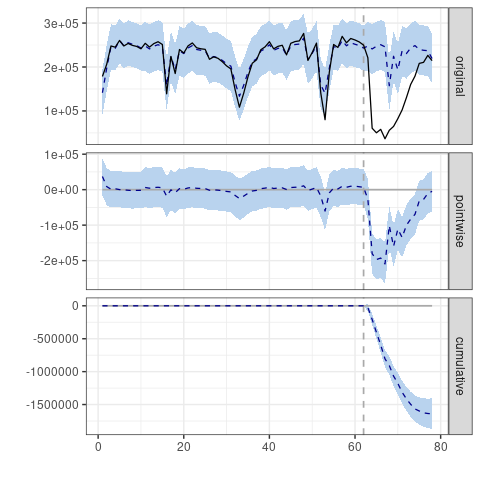
\includegraphics[width=9cm]{global_covid.png}\caption{Estimación del impacto de la pandemia sobre el número semanal de actos médicos.}
      \end{figure}\label{global_covid}
      \end{center}

Los resultados de la tabla anterior muestran una reducción significativa estimada en un 44\% del número semanal global de actos médicos en el periodo de confinamiento, y un aumento significativo en el periodo post-pandemia, tanto en la definición del escenario 1 como en el escenario 2 (que excluye del periodo post-covid el periodo de confinamiento domiciliario comprendido entre el 14-03-2020 y el 21-06-2020), estimado en el 18\% y el 10\% respectivamente.
      
  \begin{center}
  \begin{figure}[H]
    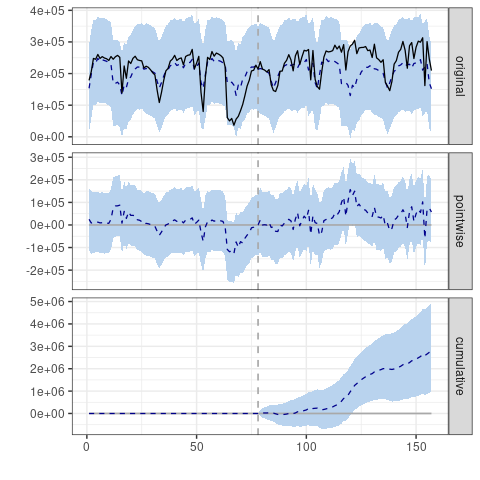
\includegraphics[width=9cm]{global_post_scen1.png}\caption{Estimación del impacto de la post-pandemia sobre el número semanal de actos médicos según el escenario 1.}\label{global_postcovid1}
  \end{figure}
  \end{center}
  
  \begin{center}
      \begin{figure}[H]
        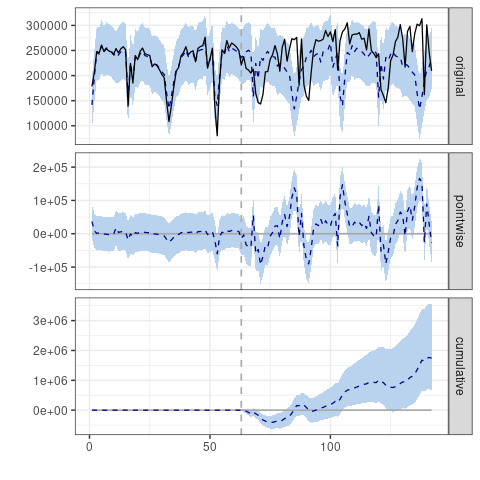
\includegraphics[width=9cm]{global_post_scen2.png}\caption{Estimación del impacto de la post-pandemia sobre el número semanal de actos médicos según el escenario 2.}\label{global_postcovid2}
      \end{figure}
      \end{center}

En las figuras~\ref{global_postcovid1} y~\ref{global_postcovid2} puede verse el aumento significativo en el periodo post-covid en cualquiera de los dos escenarios considerados.

%%%Resultats de obstetrics globalment
\begin{table}[H]\caption{Estimación del impacto de la pandemia sobre el número semanal de visitas al servicio de obstetricia.}
    \centering  
    \begin{tabular}{ |c|c|c|c| }
        \hline
        \textbf{Escenario} & \textbf{Periodo} & \textbf{Efecto relativo (s.d.)} & \textbf{Prob. de efecto causal} \\ 
        \hline
     1 & Covid-19 & -46\% (1.7\%) & 99.99\% \\  
     1 & Post-covid & 17\% (9.5\%) & 98.54\% \\
     \hline   
     2 & Post-covid & 9\% (4.3\%) & 98.52\% \\
     \hline
    \end{tabular}
  \end{table}
  
  \begin{center}
    \begin{figure}[H]
      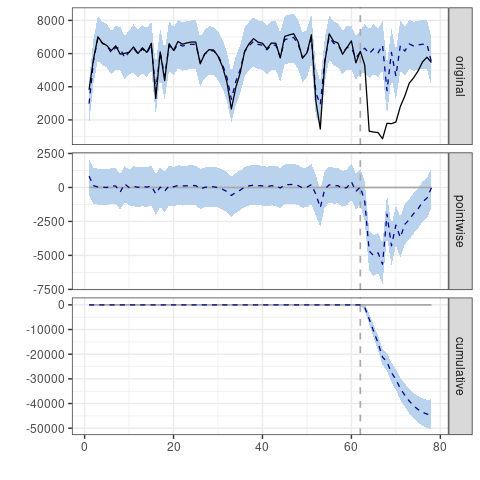
\includegraphics[width=9cm]{obstetrics_covid.png}\caption{Estimación del impacto de la pandemia sobre el número semanal de visitas al servicio de obstetricia.}
    \end{figure}
    \end{center}
    
  \begin{center}
  \begin{figure}[H]
  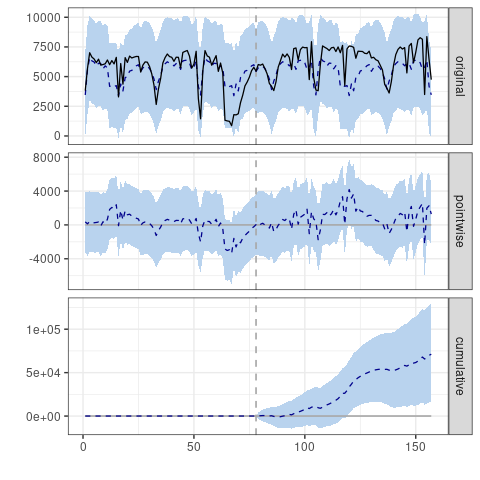
\includegraphics[width=9cm]{obstetrics_post_scen1.png}\caption{Estimación del impacto de la post-pandemia sobre el número semanal de visitas al servicio de obstetricia según el escenario 1.}
  \end{figure}
  \end{center}
  
  \begin{center}
    \begin{figure}[H]
      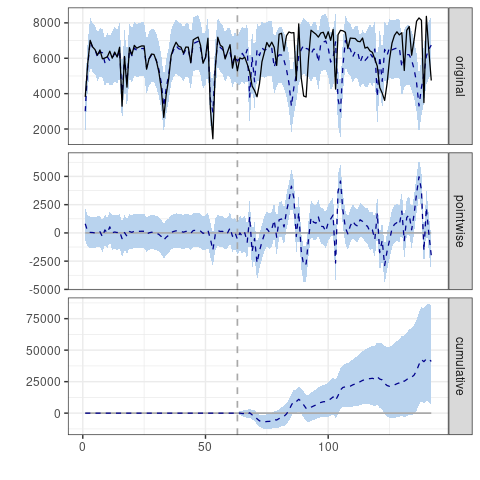
\includegraphics[width=9cm]{obstetrics_post_scen2.png}\caption{Estimación del impacto de la post-pandemia sobre el número semanal de visitas al servicio de obstetricia según el escenario 2.}
    \end{figure}
    \end{center}

De manera similar a lo descrito anteriormente, si analizamos exclusivamente la serie temporal del número semanal de visitas al servicio de obstetricia, se observa también una dismunición significativa, de alrededor del 46\% en el periodo de confinamiento domiciliario, y un aumento significativo alrededor del 17\% o del 9\% en el periodo post-covid, según los escenarios 1 y 2 respectivamente. 
    
\subsubsection{Madrid}\label{madrid}
\begin{table}[H]\caption{Estimación del impacto de la pandemia y post-pandemia sobre el número semanal de actos médicos en Madrid.}
    \centering  
      \begin{tabular}{ |c|c|c|c| }
          \hline
          \textbf{Escenario} & \textbf{Periodo} & \textbf{Efecto relativo (s.d.)} & \textbf{Prob. de efecto causal} \\ 
          \hline
       1 & Covid-19 & -48\% (1.7\%) & 99.99\% \\  
       1 & Post-covid & 9.2\% (11\%) & 92\% \\
       \hline   
       2 & Post-covid & 1.9\% (4.6\%) & 70\% \\
       \hline
      \end{tabular}
  \end{table}
  
  \begin{center}
      \begin{figure}[H]
        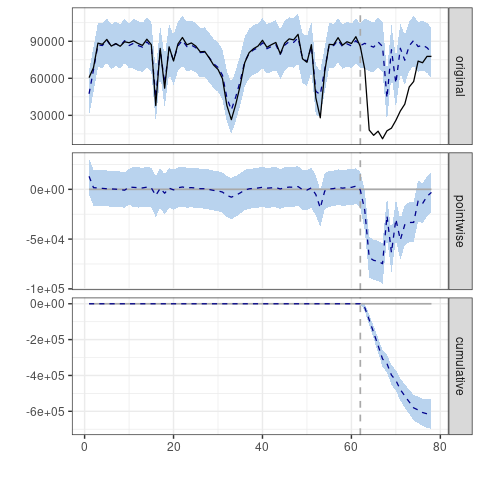
\includegraphics[width=9cm]{global_covid_Madrid.png}\caption{Estimación del impacto de la pandemia sobre el número semanal de actos médicos en Madrid.}
      \end{figure}
      \end{center}
      
  \begin{center}
  \begin{figure}[H]
    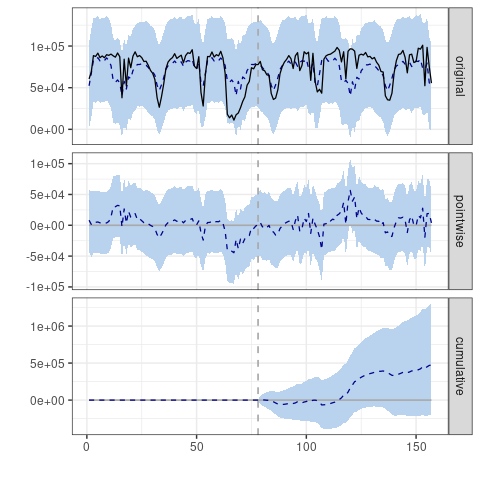
\includegraphics[width=9cm]{global_post_scen1_Madrid.png}\caption{Estimación del impacto de la post-pandemia sobre el número semanal de actos médicos según el escenario 1 en Madrid.}
  \end{figure}
  \end{center}
  
  \begin{center}
      \begin{figure}[H]
        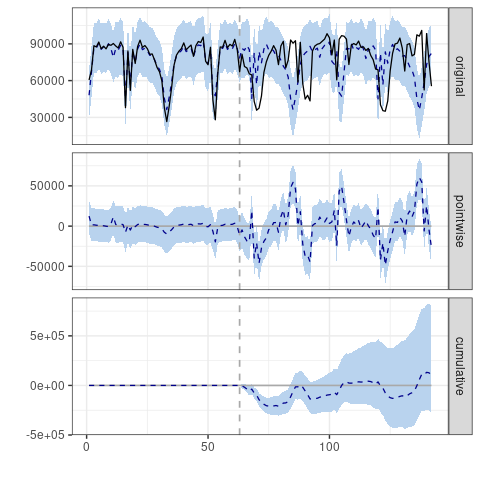
\includegraphics[width=9cm]{global_post_scen2_Madrid.png}\caption{Estimación del impacto de la post-pandemia sobre el número semanal de actos médicos según el escenario 2 en Madrid.}
      \end{figure}
      \end{center}

Los resultados muestran que en Madrid, en la línea de lo descrito en el apartado anterior, se observa una disminución significativa en el número semanal de actos médicos en el periodo de confinamiento domiciliario (estimada alrededor del 48\%), pero contrariamente a lo descrito previamente, el aumento posterior (estimado en un 9.2\% y 1.9\% para los escenarios 1 y 2 respectivamente) no resulta significativamente atribuible a las consecuencias de la pandemia.      
%%% Resultats de obstetrics a Madrid
\begin{table}[H]\caption{Estimación del impacto de la pandemia sobre el número semanal de visitas al servicio de obstetricia en Madrid.}
    \centering
      \begin{tabular}{ |c|c|c|c| }
        \hline
        \textbf{Escenario} & \textbf{Periodo} & \textbf{Efecto relativo (s.d.)} & \textbf{Prob. de efecto causal} \\ 
        \hline
     1 & Covid-19 & -51\% (1.4\%) & 99.99\% \\  
     1 & Post-covid & 11\% (9.9\%) & 94\% \\
     \hline   
     2 & Post-covid & 2.6\% (4.3\%) & 79\% \\
     \hline
    \end{tabular}
  \end{table}
  
  \begin{center}
    \begin{figure}[H]
      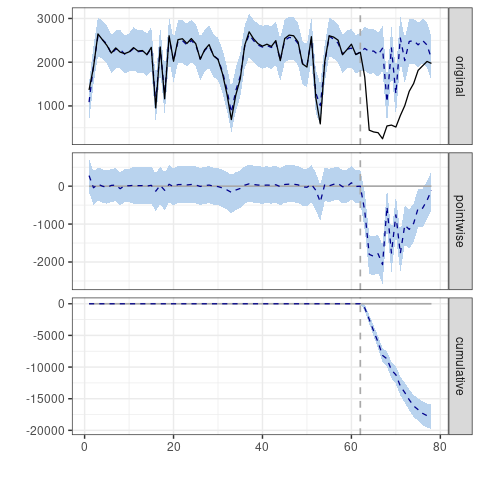
\includegraphics[width=9cm]{obstetrics_covid_Madrid.png}\caption{Estimación del impacto de la pandemia sobre el número semanal de visitas al servicio de obstetricia en Madrid.}
    \end{figure}
    \end{center}
    
  \begin{center}
  \begin{figure}[H]
  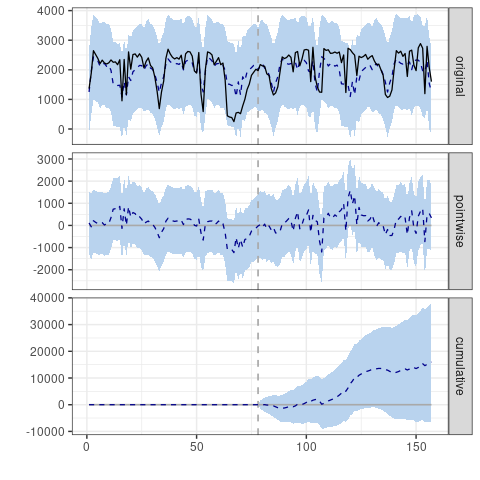
\includegraphics[width=9cm]{obstetrics_post_scen1_Madrid.png}\caption{Estimación del impacto de la post-pandemia sobre el número semanal de visitas al servicio de obstetricia según el escenario 1 en Madrid.}
  \end{figure}
  \end{center}
  
  \begin{center}
    \begin{figure}[H]
      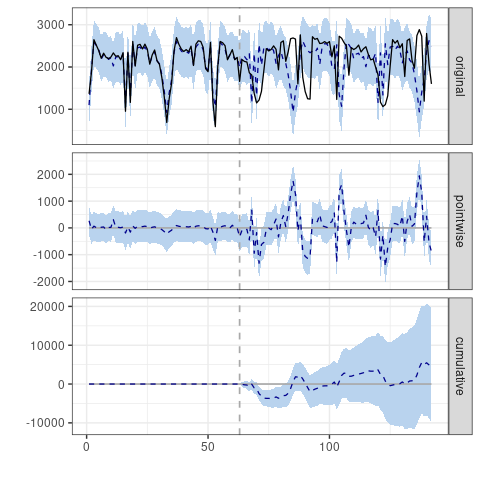
\includegraphics[width=9cm]{obstetrics_post_scen2_Madrid.png}\caption{Estimación del impacto de la post-pandemia sobre el número semanal de visitas al servicio de obstetricia según el escenario 2 en Madrid.}
    \end{figure}
    \end{center}

Respecto al análisis de la evolución del número semanal de visitas al servicio de obstetricia en la provincia de Madrid, los resultados muestran que en Madrid, en la línea de lo descrito en el apartado anterior, se observa una disminución significativa en el número semanal de actos médicos en el periodo de confinamiento domiciliario (estimada alrededor del 48\%), pero contrariamente a lo descrito previamente, el aumento posterior (estimado en un 9.2\% y 1.9\% para los escenarios 1 y 2 respectivamente) no resulta significativamente atribuible a las consecuencias de la pandemia.      

\subsubsection{Barcelona}\label{bcn}
\begin{table}[H]\caption{Estimación del impacto de la pandemia y post-pandemia sobre el número semanal de actos médicos en Barcelona.}
    \centering  
    \begin{tabular}{ |c|c|c|c| }
        \hline
        \textbf{Escenario} & \textbf{Periodo} & \textbf{Efecto relativo (s.d.)} & \textbf{Prob. de efecto causal} \\ 
        \hline
     1 & Covid-19 & -46\% (2.2\%) & 99.99\% \\  
     1 & Post-covid & 26\% (13\%) &  99.66\% \\
     \hline   
     2 & Post-covid & 16\% (4.8\%) & 99.77\% \\
     \hline
    \end{tabular}
  \end{table}
  
  \begin{center}
    \begin{figure}[H]
      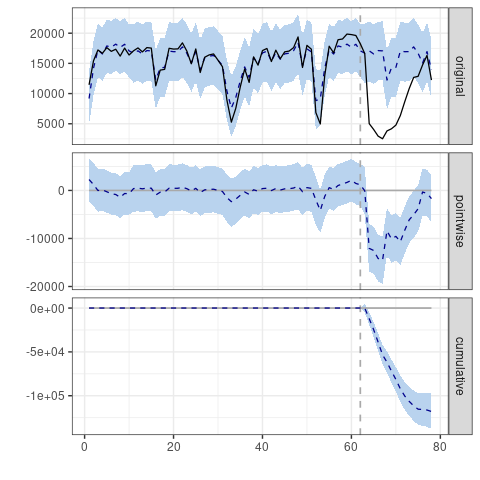
\includegraphics[width=9cm]{global_covid_Barcelona.png}\caption{Estimación del impacto de la pandemia sobre el número semanal de actos médicos en Barcelona.}
    \end{figure}
    \end{center}
    
  \begin{center}
  \begin{figure}[H]
  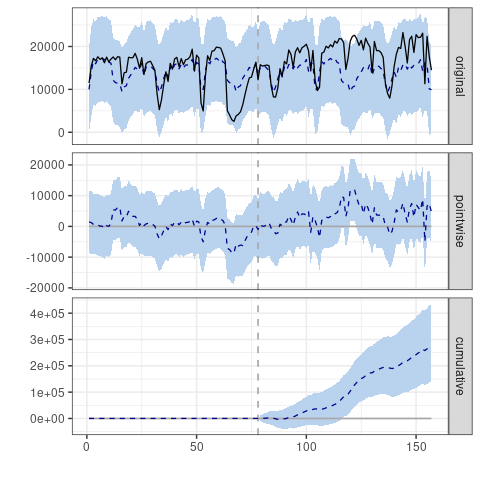
\includegraphics[width=9cm]{global_post_scen1_Barcelona.png}\caption{Estimación del impacto de la post-pandemia sobre el número semanal de actos médicos según el escenario 1 en Barcelona.}
  \end{figure}
  \end{center}
  
  \begin{center}
    \begin{figure}[H]
      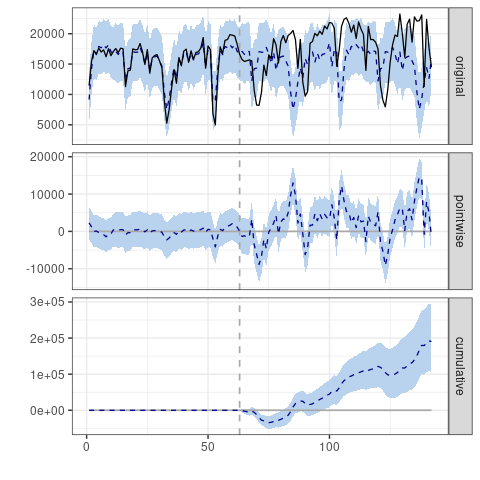
\includegraphics[width=9cm]{global_post_scen2_Barcelona.png}\caption{Estimación del impacto de la post-pandemia sobre el número semanal de actos médicos según el escenario 2 en Barcelona.}
    \end{figure}
    \end{center}

Los resultados muestran que en la provincia de Barcelona, en la línea de lo que ocurre globalmente, se observa una disminución significativa en el número semanal de actos médicos en el periodo de confinamiento domiciliario (estimada alrededor del 46\%), y el aumento posterior (estimado en un 26\% y 16\% para los escenarios 1 y 2 respectivamente) resulta también atribuible a las consecuencias de la pandemia de forma significativa.

%%% Resultats de obstetrics a Barcelona
\begin{table}[H]\caption{Estimación del impacto de la pandemia sobre el número semanal de visitas al servicio de obstetricia en Barcelona.}
    \centering  
    \begin{tabular}{ |c|c|c|c| }
        \hline
        \textbf{Escenario} & \textbf{Periodo} & \textbf{Efecto relativo (s.d.)} & \textbf{Prob. de efecto causal} \\ 
        \hline
     1 & Covid-19 & -43\% (2.3\%) & 99.99\% \\  
     1 & Post-covid & 24\% (9.2\%) & 99.53\% \\
     \hline   
     2 & Post-covid & 17\% (5\%) & 99.53\% \\
     \hline
    \end{tabular}
  \end{table}
  
  \begin{center}
    \begin{figure}[H]
      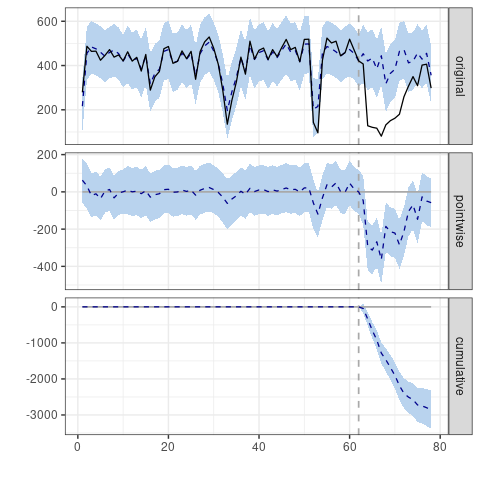
\includegraphics[width=9cm]{obstetrics_covid_Barcelona.png}\caption{Estimación del impacto de la pandemia sobre el número semanal de visitas al servicio de obstetricia en Barcelona.}
    \end{figure}
    \end{center}
    
  \begin{center}
  \begin{figure}[H]
  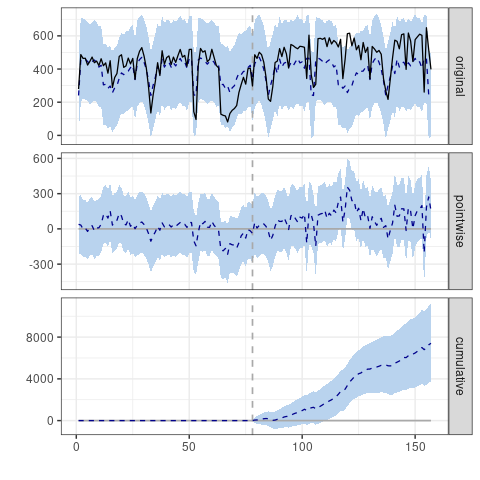
\includegraphics[width=9cm]{obstetrics_post_scen1_Barcelona.png}\caption{Estimación del impacto de la post-pandemia sobre el número semanal de visitas al servicio de obstetricia según el escenario 1 en Barcelona.}
  \end{figure}
  \end{center}
  
  \begin{center}
    \begin{figure}[H]
      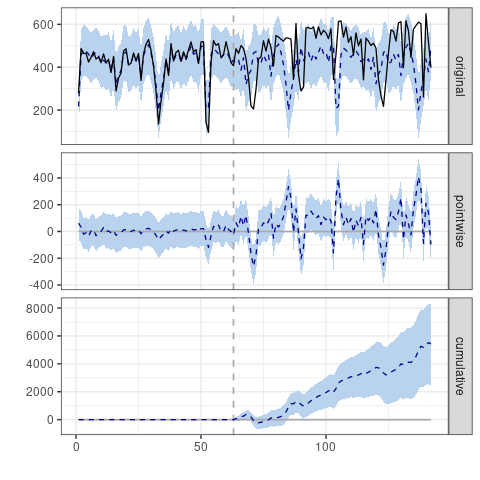
\includegraphics[width=9cm]{obstetrics_post_scen2_Barcelona.png}\caption{Estimación del impacto de la post-pandemia sobre el número semanal de visitas al servicio de obstetricia según el escenario 2 en Barcelona.}
    \end{figure}
    \end{center}

Respecto al análisis de la evolución del número semanal de visitas al servicio de obstetricia en la provincia de Barcelona, los resultados muestran que, en la línea de lo descrito anteriormente, se observa una disminución significativa en el número semanal de actos médicos en el periodo de confinamiento domiciliario (estimada alrededor del 43\%) y el aumento posterior (estimado en un 24\% y 17\% para los escenarios 1 y 2 respectivamente) resulta también atribuible a las consecuencias de la pandemia de forma significativa.      

\subsubsection{Valencia}\label{valencia}
\begin{table}[H]\caption{Estimación del impacto de la pandemia y post-pandemia sobre el número semanal de actos médicos en Valencia.}
    \centering  
    \begin{tabular}{ |c|c|c|c| }
        \hline
     \textbf{Escenario} & \textbf{Periodo} & \textbf{Efecto relativo (s.d.)} & \textbf{Prob. de efecto causal} \\ 
     \hline
     1 & Covid-19 & -41\% (2.1\%) & 99.99\% \\  
     1 & Post-covid & 28\% (10\%) &  99.83\% \\
     \hline   
     2 & Post-covid & 21\% (4.8\%) & 99.99\% \\
     \hline
    \end{tabular}
  \end{table}
  
  \begin{center}
    \begin{figure}[H]
      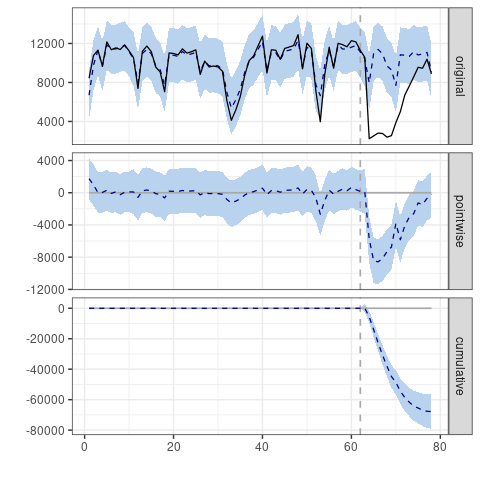
\includegraphics[width=9cm]{global_covid_Valencia.png}\caption{Estimación del impacto de la pandemia sobre el número semanal de actos médicos en Valencia.}
    \end{figure}
    \end{center}
    
  \begin{center}
  \begin{figure}[H]
  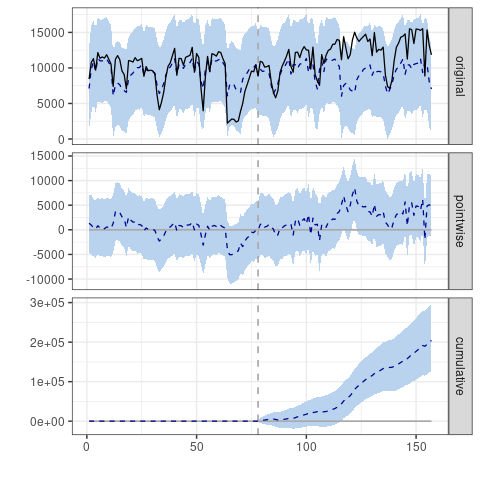
\includegraphics[width=9cm]{global_post_scen1_Valencia.png}\caption{Estimación del impacto de la post-pandemia sobre el número semanal de actos médicos según el escenario 1 en Valencia.}
  \end{figure}
  \end{center}
  
  \begin{center}
    \begin{figure}[H]
      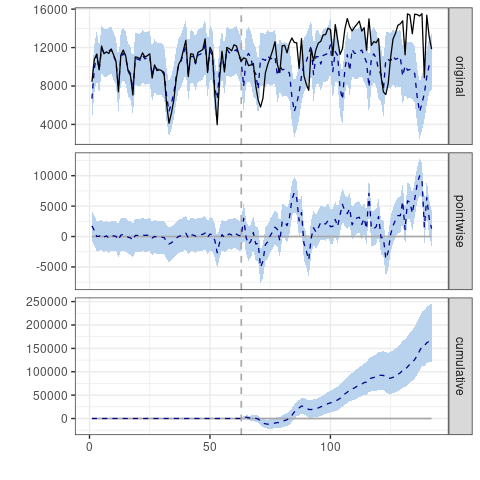
\includegraphics[width=9cm]{global_post_scen2_Valencia.png}\caption{Estimación del impacto de la post-pandemia sobre el número semanal de actos médicos según el escenario 2 en Valencia.}
    \end{figure}
    \end{center}

Los resultados muestran que en la provincia de Valencia, en la línea de lo que ocurre globalmente, se observa una disminución significativa en el número semanal de actos médicos en el periodo de confinamiento domiciliario (estimada alrededor del 41\%), y el aumento posterior (estimado en un 28\% y 21\% para los escenarios 1 y 2 respectivamente) resulta también atribuible a las consecuencias de la pandemia de forma significativa.

%%% Resultats de obstetrics a Valencia
\begin{table}[H]\caption{Estimación del impacto de la pandemia sobre el número semanal de visitas al servicio de obstetricia en Valencia.}
    \centering
      \begin{tabular}{ |c|c|c|c| }
          \hline
          \textbf{Escenario} & \textbf{Periodo} & \textbf{Efecto relativo (s.d.)} & \textbf{Prob. de efecto causal} \\ 
          \hline
       1 & Covid-19 & -42\% (2.5\%) & 99.99\% \\  
       1 & Post-covid & 32\% (9.1\%) & 99.78\% \\
       \hline   
       2 & Post-covid & 24\% (5\%) & 99.89\% \\
       \hline
      \end{tabular}
    \end{table}
    
    \begin{center}
      \begin{figure}[H]
        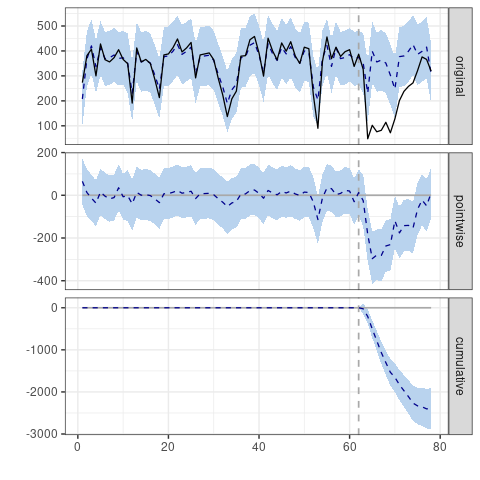
\includegraphics[width=9cm]{obstetrics_covid_Valencia.png}\caption{Estimación del impacto de la pandemia sobre el número semanal de visitas al servicio de obstetricia en Valencia.}
      \end{figure}
      \end{center}
      
    \begin{center}
    \begin{figure}[H]
    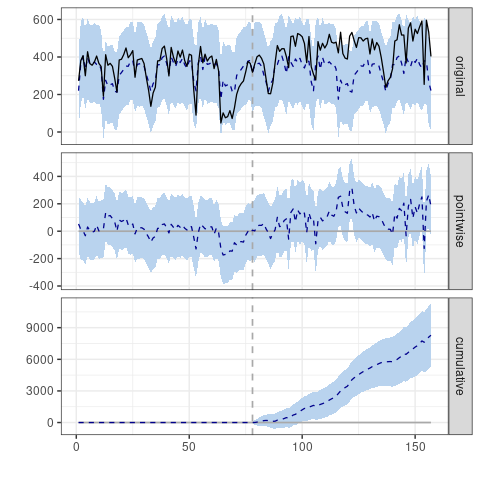
\includegraphics[width=9cm]{obstetrics_post_scen1_Valencia.png}\caption{Estimación del impacto de la post-pandemia sobre el número semanal de visitas al servicio de obstetricia según el escenario 1 en Valencia.}
    \end{figure}
    \end{center}
    
    \begin{center}
      \begin{figure}[H]
        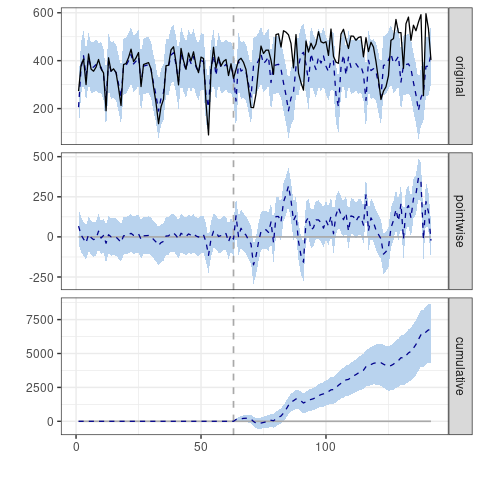
\includegraphics[width=9cm]{obstetrics_post_scen2_Valencia.png}\caption{Estimación del impacto de la post-pandemia sobre el número semanal de visitas al servicio de obstetricia según el escenario 2 en Valencia.}
      \end{figure}
      \end{center}

Respecto al análisis de la evolución del número semanal de visitas al servicio de obstetricia en la provincia de Valencia, los resultados muestran que, en la línea de lo descrito anteriormente, se observa una disminución significativa en el número semanal de actos médicos en el periodo de confinamiento domiciliario (estimada alrededor del 42\%) y el aumento posterior (estimado en un 32\% y 24\% para los escenarios 1 y 2 respectivamente) resulta también atribuible a las consecuencias de la pandemia de forma significativa.  

\section{Discusión}


\section{Actividades realizadas en el marco del Proyecto}
\subsection{Contribuciones en congresos nacionales e internacionales}
\begin{enumerate}
  \item Estimated Covid-19 burden in Spain: ARCH underreported non-stationary time series. \textbf{David Moriña}, Amanda Fernández-Fontelo, Alejandra Cabaña, Argimiro Arratia, Pedro Puig. Contribución oral presentada en el 36 International Workshop on Statistical Modelling celebrada en Trieste (Italia) entre el 18 y el 22 de Julio de 2022.
  \item A new statistical model to assess the burden of misreported epidemiological data. \textbf{David Moriña}, Amanda Fernández-Fontelo, Alejandra Cabaña, Argimiro Arratia, Pedro Puig. Contribución oral presentada en la reunión anual de la Sociedad Española de Epidemiología (SEE), celebrada en Donosti (España) entre el 30 de Agosto de 2022 y el 2 de Septiembre de 2022.
  \item Impact of Covid-19 pandemic in health services usage. \textbf{David Moriña}, Amanda Fernández-Fontelo, Pere Puig, Montserrat Guillen. Contribución oral invitada presentada en el primer UB School of Economics Young Research Meeting, celebrado en Barcelona el 22 de Septiembre de 2022. 
  \item Modelling the impact of Covid-19 pandemics on health insurance associated services demand. \textbf{Amanda Fernández-Fontelo}, Pedro Puig, Montserrat Guillén, David Moriña. Contribución oral presentada en el 8 Workshop on Risk Management and Insurance Research (RISK 2022), celebrado en Barcelona entre el 20 y el 21 de Octubre de 2022.
  \item Reunión de coordinadores de la red nacional de Bioestadística BioStatNeXt, celebrada en Valencia el 9 y 10 de Marzo de 2023. Difusión de resultados.
\end{enumerate}
  
\subsection{Articulos científicos}
\begin{enumerate}
\item David Moriña. Impact of the Covid-19 pandemic in health services usage. Boletín de la Sociedad Española de Estadística e Investigación Operativa, 7 (2022). \url{https://www.seio.es/wp-content/uploads/2022/07/Julio2022_Estadistica.pdf}
\item David Moriña, Amanda Fernández-Fontelo, Alejandra Cabaña, Argimiro Arratia, Pedro Puig. Estimated Covid-19 burden in Spain: ARCH underreported non-stationary time series. BMC Medical Research Methodology (Accepted)
\item Amanda Fernández-Fontelo, Pedro Puig, David Moriña. Modelling the impact of Covid-19 pandemics on health insurance associated services demand. (In preparation).
\item David Moriña, Amanda Fernández-Fontelo, Montserrat Guillén. Overuse of private healthcare insurance services after the Covid-19 pandemic. (In preparation).
\end{enumerate}

\section{Memoria económica}

\section*{Certificados de participación}
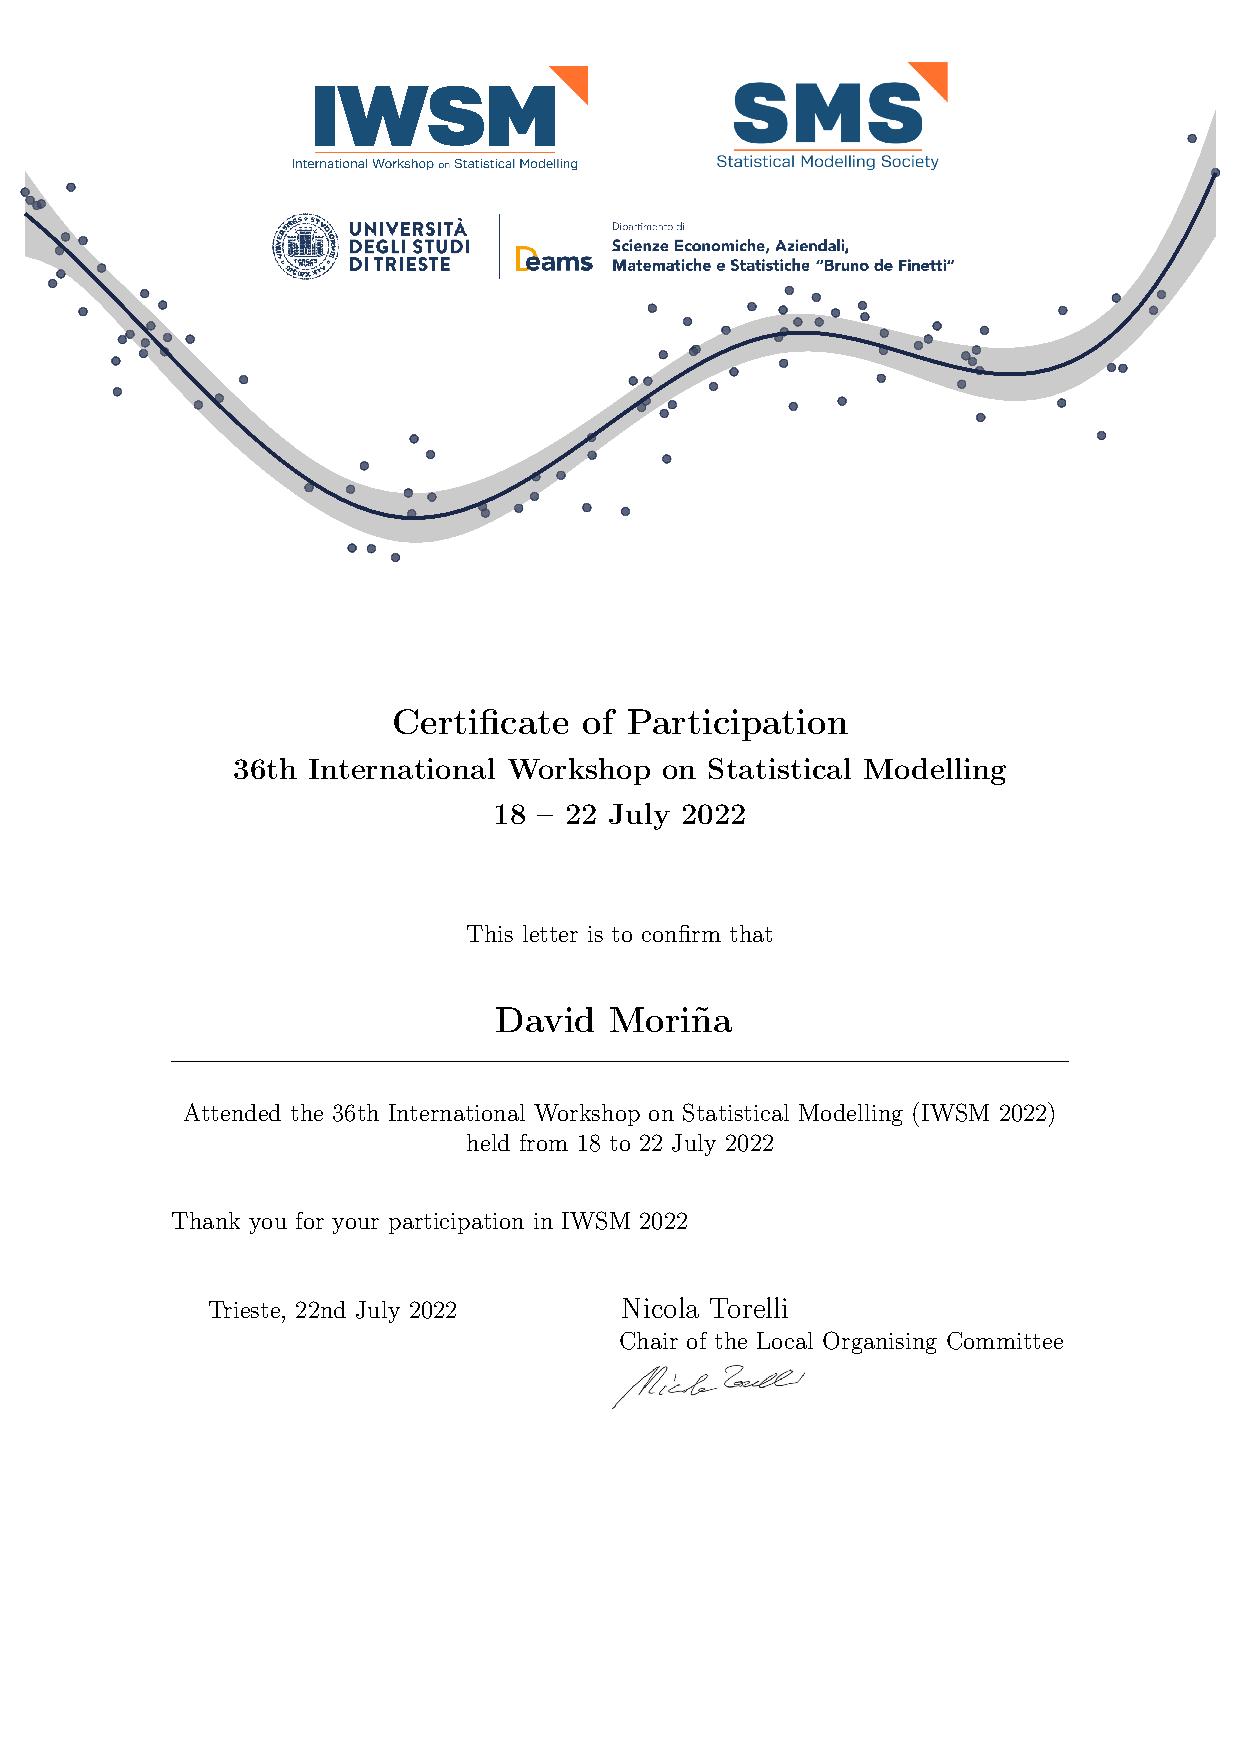
\includepdf[pages=-]{Annex/CertificateIWSM2022MorinaDavid.pdf}
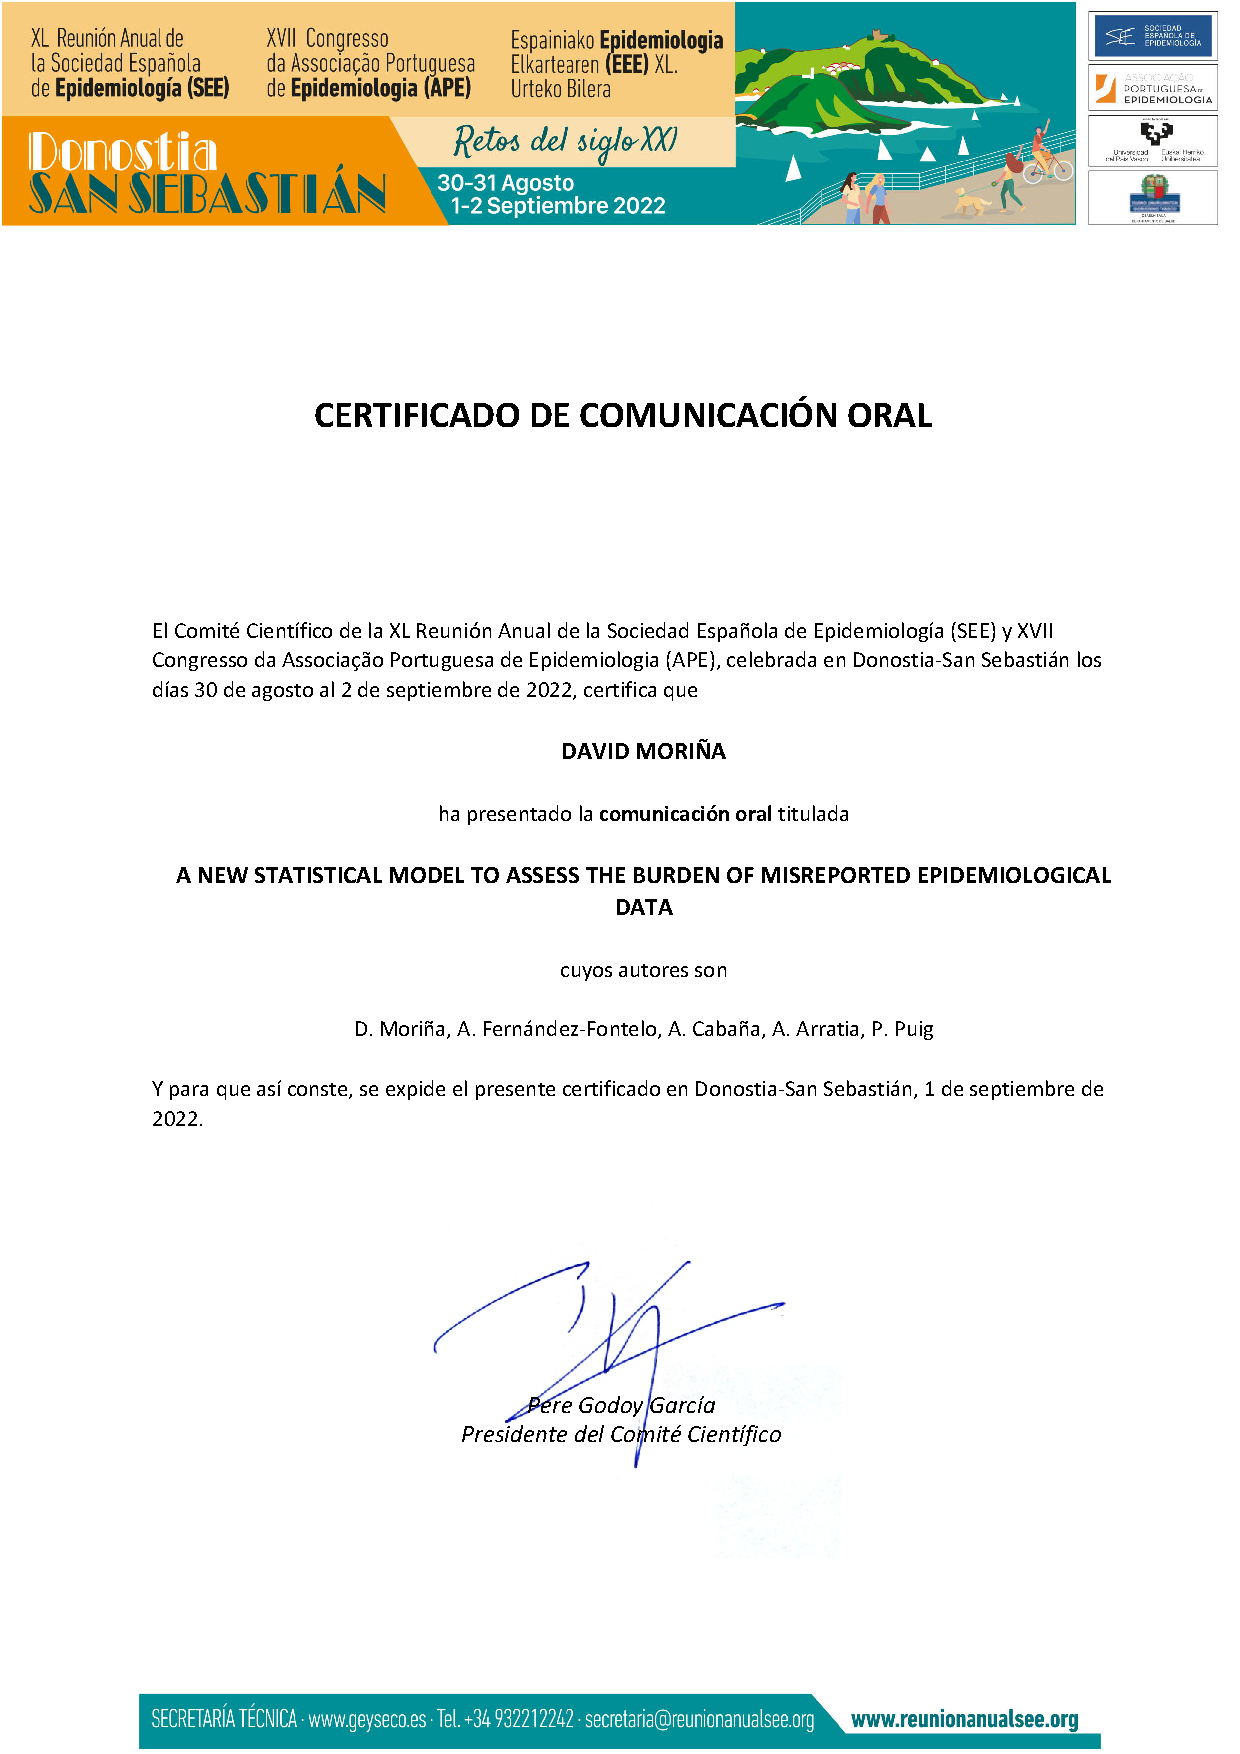
\includepdf[pages=-]{Annex/C-141.pdf}
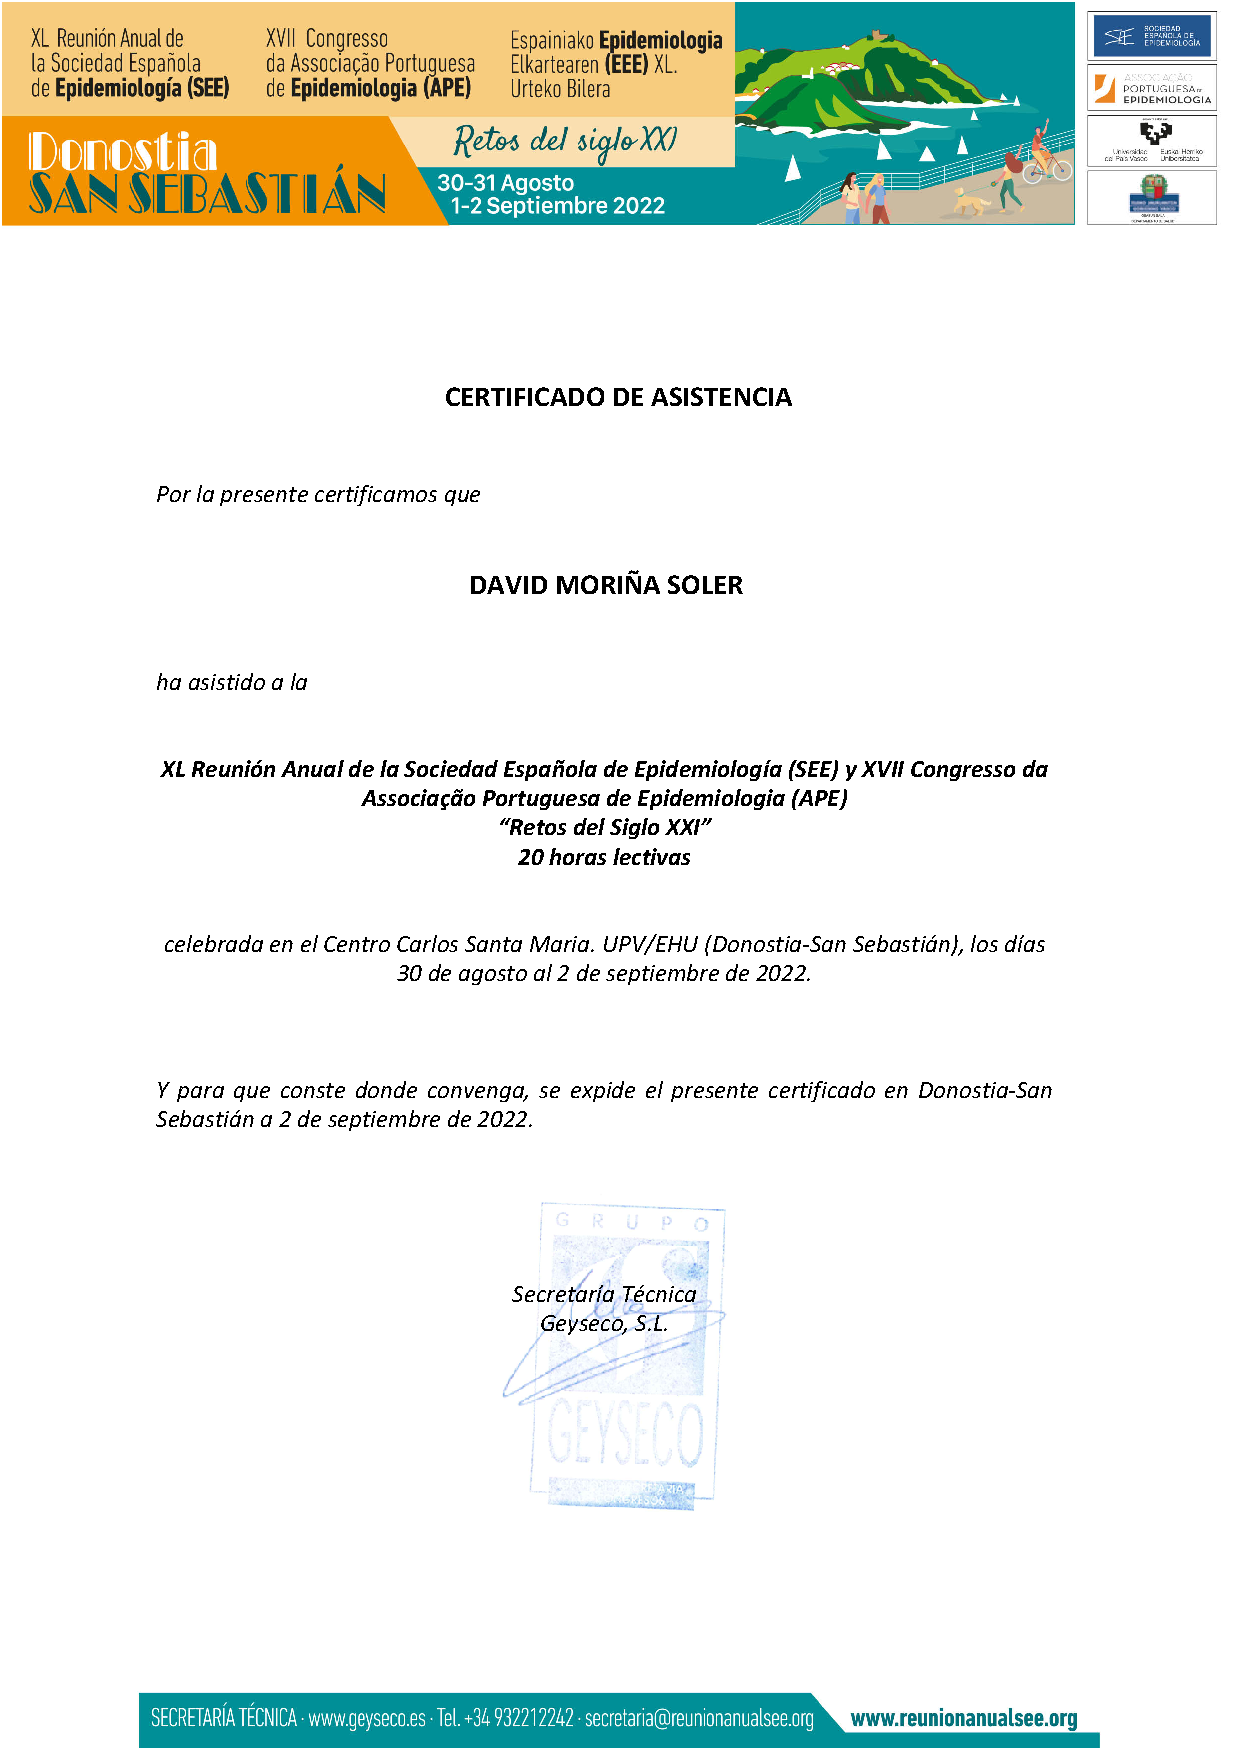
\includepdf[pages=-]{Annex/MORIÑA SOLER.pdf}

% Bibliography.
% -------------
\parskip=0pt
\parsep=0pt
\bibliographystyle{ieeetrsrt}

% Important: substitute your BiBTeX (*.bib) files below.
% ------------------------------------------------------
\bibliography{report}

\end{document}
